
\documentclass{article}
\title{Research Internship Report}
\author{}
\date{}

\usepackage[utf8]{inputenc}
\usepackage{mathtools}
\usepackage{amsfonts}
\usepackage{amsthm}
\usepackage{relsize}
\usepackage{dsfont} 
\usepackage[all]{xy}
\usepackage{float}
\usepackage{color}
\usepackage{comment}
\usepackage{pdfpages}
\usepackage{titling}
\usepackage{stmaryrd}
\usepackage{appendix}
\usepackage{graphicx,fancyhdr,mwe}

\usepackage[a4paper,margin=2.5cm,bottom=2cm,headheight=2cm]{geometry}
\pagestyle{fancy}
\fancyhead[LO,RE]{\includegraphics[scale=0.2]{ucdavislogo.eps}}
\cfoot{\thepage}
\rfoot{\includegraphics[scale=1]{logoX.jpg}}


\renewcommand{\maketitlehooka}{\'ECOLE POLYTECHNIQUE\newline
 
Promotion X2014 \newline

Ma\"el FORCIER}

\newcommand{\mf}[1]{\textcolor{red}{$\textrm{Mael: }${#1}}}
\newcommand{\code}[2]{\texttt{#1}}

\begin{document}

\includepdf[pages=-]{front_page.pdf}
   \includepdf[pages=-,pagecommand={\thispagestyle{plain}}]{declaration_integrite.pdf}
   \vspace*{\stretch{0.7}}
   \section*{Abstract}
   \textit{
   In my internship at the University of California in Davis, I worked on a software that creates scenarios for the production of solar and wind renewable energy to use them in a stochastic optimization problem of unit commitment. This software is called} \texttt{Prescient} \textit{and it is used by researchers at Universities and the US Department of Energy and may eventually be used by grid operators. To do so, we need to analyze the actual powers and the errors to the forecast power that are produced and especially the dependence of these values between different hours of the day. I then coded in} \texttt{Prescient} \textit{a complex tool that allow any user to work with multidimensional random variables and their distributions and especially to use copulas which are useful tools to capture the dependence between random variables without focusing on the univariate distributions of the coordonates called marginals. I explain in this report how this code is structured, the way it was designed and how to use it. Then, I used this code to make some experiments with real data of wind energy production. Inspired by the litterature and the previous interns, I created a method and an algorithm that permits to check how well a copula fits the datas. The mathematical aspects of this method and the algorithm are also presented here. I eventually present, interpret and comment the results I obtained. All copulas seem to fit pretty well the data except for the independence copula which does not fit them at all as we expected.}
   \vspace*{\stretch{0.5}}
   \section*{Résumé}
   \textit{
   Lors de ce stage à l'Université de Californie de Davis, j'ai travaillé sur un projet de logiciel qui crée des scénarios de production d'énergies renouvelables solaires et éoliennes pour les utiliser dans un problème d'optimisation stochastique. Ce logiciel nommé} \texttt{Prescient} \textit{est utilisé par le US Department of Energy Pour y parvenir, nous devons analyser les données des puissances mesurées réellement ainsi que les erreurs ou différences par rapport aux prédictions et en particulier les corrélations de ces puissances à différentes heures de la journée. J'ai alors codé dans} \texttt{Prescient} \textit{un outil complexe qui permet à n'importe quel utilisateur de manipuler des variables aléatoires à plusieurs dimensions et leurs distributions de probabilité et surtout d'utiliser des copules qui sont des outils utiles pour étudier la dépendance entre des variables aléatoires sans se préoccuper des distributions unidimensionnelles de leurs coordonnées appelées marges. J'explique dans ce rapport comment le code est structuré, la façon dont il a été pensé et comment l'utiliser. J'ai ensuite utilisé ce code pour effectuer des expériences avec des données réelles de production d'énergie éolienne. Inspiré par la littérature et par mes prédécesseurs stagiaires, j'ai imaginé une méthode et un algorithme qui permettent de vérifier à quel point une copule décrit bien les données. Les aspects mathématiques de cette méthode et cet algorithme sont aussi présentés ici. Enfin, je présente, commente et interprète les résultats obtenus. Toutes les copules semblent bien décrire les données sauf la copule d'indépendance qui est très mauvaise comme attendu.}
   \vspace*{\stretch{1}}
   \newpage
   \vspace*{\stretch{1}}
   \section*{Acknowledgments}
   \begin{itemize}
   \item
   I would like to give sincere thanks to my mentor Professor David L. Woodruff, who guided me a lot for this job and was always a great help during this internship.
   \item
   I also want to thank my teacher, Professor St\'ephane Gaubert who made me like optimization and helped me find this internship.
   \item
   I eventually want to thank all my colleagues, Sebastian Angerhausen, Antoine Keller and Dominic Yang. It was a pleasure to work with them.
   
   \end{itemize}
   \vspace*{\stretch{1}}
   \newpage
   
   \tableofcontents

   \newpage
   \section*{Introduction}
   \addcontentsline{toc}{section}{Introduction}
	
   
	Matching the supply and the demand of energy and in particular electricity is a complex problem for the grid operators. It is usually solved in part using what is called unit commitment. Unit commitment is an optimization problem where the grid operator has to decide whether to turn on or off each unit of electricity production so that the demand is matched. That means providing enough energy so that every client can use the energy he wants and not providing too much energy which will implies insecurity on the network as well as a loss of energy and money. Unit commitments were historically deterministic problems where the production and the demand are reliable forecast. Nevertheless, in the last decade, the production of electricity with renewable energies especially wind and solar energies has significantly increase in California and all over the world. These new sources are intermittent and less predictable, unit commitment problems then become stochastic. The more the part of solar and wind is in the electricity generation is, the harder it will be to forecast the production and to take the best unit commitment decisions.\newline
	
	\begin{figure}[h]
	\centering  
    \includegraphics[width=0.7\textwidth]{CAISO-Bar-Chart.png}
    \caption{Electricity production from different sources between 2012 and 2015}
\end{figure}
	
	Professor David L.Woodruff from the University of California at Davis and his team are working on a software in python called \texttt{Prescient} providing solutions for stochastic unit commitment problems for electricity grid management companies such as California Independent System Operator (CAISO) or power marketing agencies such as Bonneville Power Association (BPA). In order to have accurate and efficient solutions to stochastic optimization problems, instead of a deterministic forecast, we have to  create different scenarios with their probabilities to happen. The project I was working in was called Grid Operation Scenario Maker (GOSM). Its goal was to provide relevant scenarios and probabilities that could be used by the stochastic optimization algorithm of prescient.
	
	When I started my internship, GOSM was already able to create scenarios of wind and solar energy production by focusing on the errors between the forecast power and the actual power that was measured. The probabilities were calculated thanks to error distributions at different hours of the day called day part separators. However, the random variables representing the different sources at different dps were considered independent because it was first easier to code. But, it seems obvious that the energy production or the errors  between two adjacent hours are highly correlated. Moreover, nothing tells us that the energy production of wind and solar are not correlated. Because GOSM had already integrated the distribution of this variable, the best way to modelize the dependance between variables without caring about the distribution of each variable which we call marginals is to use copulas. Copulas are useful mathematical tools which only describes the dependance between variables and which do not depend of marginals. My work in the GOSM team was to implement different kinds of copulas in the software and to test on various datas how well they modelize the dependence between the datas. In this report, I will first explain how I built this distribution and copula library for GOSM in python. Then, I will present the experiment I did to verify how copulas fit the datas. I will finally show and analyze the result I found.
	
	\newpage
	
	\section{Distribution and copula library}
	
	The first part of my job was to create copula classes that were easy and intuitive to use for other users such as the next people who will work on GOSM. At the beginning of my internship only 2 distribution classes(\texttt{UnivariateEmpiricalDistribution}, \texttt{UnivariateEpiSplineDistribution}) were implemented. To make verifications and control tests, I had to implement other classical distributions in addition to copulas. At the end, I had a great and pretty complete library of distributions and copulas with a relevant object oriented structure. I wrote a user manual to explain how this library works. This section sums up this user manual. If more details are needed, you can find the whole formulas in the Appendix~\ref{sec:list},~\ref{sec:distributions} and~\ref{sec:copulas}.
	
	\subsection{Mathematical Definitions}
	\newtheorem{definition}{Definition}
	\newtheorem{property}{Property}
	\begin{definition}
	The cumulative density function (cdf) of a random variable $X \in \mathbb{R}$ is the function $F : \mathbb{R} \to [0,1]$ where :
	\begin{equation*}
	F(x) = \mathbb{P}(X\leq x)
	\end{equation*}	
	\end{definition}
	
	This definition also works when X is a multidimensional random	variable i.e. $\in \mathbb{R}^d$ if we use the notation $(x_1,...,x_d) \leq (y_1,...,y_d) \Leftrightarrow \forall i, x_i \leq y_i$	
	
	
	\begin{definition}
	If the cdf of $X \in \mathbb{R}$ is differentiable, the probability density function (pdf) of X is the function $f : \mathbb{R} \to [0,1]$ where :
	\begin{equation*}
	f(x) = \frac{dF(x)}{dx} = \frac{d\mathbb{P}(X\leq x)}{dx}
	\end{equation*}
	If $X \in \mathbb{R}^d$ and F is regular enough, the probability density function pdf of X is the function $f : \mathbb{R} \to [0,1]$ :
	\begin{equation*}
	f(x) = \frac{d^d F(x)}{dx_1...dx_d}
	\end{equation*}
	\end{definition}	
	
	
	
	Each one of these two functions gives all the informations about how the random variable X behaves. With them, we can compute different charasteristic values of the distribution.
	
	\begin{definition}
	The mean of a random variable $X \in \mathbb{R}^d$ is :
	\begin{equation*}
	\mathbb{E}(X) = \int_{\mathbb{R}^d} xf(x)dx
	\end{equation*}
	\end{definition} 
	
	\begin{definition}
	The variance of a random variable $X \in \mathbb{R}^d$ is :
	\begin{equation*}
	Var(X) = \mathbb{E}((X-\mathbb{E}(X))^2) = \int_{\mathbb{R}^d} (x-\mathbb{E}(X))^2f(x)dx
	\end{equation*}
	\end{definition}
	
	\begin{property}
	If $X \in \mathbb{R}$ is a random variable with a continuous cdf F,
	\begin{equation*}
	\text{then } U = F(X) \text{ is a uniform random variable in [0,1]}
	\end{equation*}
	\end{property}
	
	
	
	
	\subsection{Distributions}	
	
	To model the random properties of data (for example the production of wind power or wind forecast errors), we define distribution as a python object that contains several methods. This distribution python object does not correspond strictly to the mathematical definition of a distribution because it contains several different methods that describe many things linked to the probability law of the variable. To simplify, when we will talk about distributions, it will refer to the python objects or classes that will inherit from \texttt{BaseDistribution} class.
	
	\begin{figure}[H]
\[
   	\xymatrix{
   		 & \boxed{input\_data} \ar[dd]_{\_\_init\_\_} & \\
   		 & & \\
   		 & \boxed{parameters} \ar[ldd]_{generates\_X} \ar[rdd]^{calculus} & \\
   		 & & \\
   		\boxed{sample} \ar@/_/[rr]_{counting} & & \boxed{functions} \ar@/_/[ll]_{CDF^{-1}(Uniform\text{ }variable)}
   	}
   \]	 
   \caption{Simplified diagram of how a distribution object  works}
	\end{figure}	 
	
	\subsubsection{Methods and parameters of a distribution object}
	\paragraph{The cdf, pdf and other functions}
	The methods cdf and pdf compute the two chararacteristic functions defined above. If the object \texttt{distrobject}  represents a random variable X with cdf F and pdf f, \texttt{distrobject.cdf(x)} will return the value of $F(x)$ and \texttt{distrobject.pdf(x)} will return the value of $f(x)$. Most of the time, this value are calculated using analytical formulas.
	
	For example, the pdf of a normal distribution is calculated using the formula
	\begin{equation*}
	f(x) = \frac{1}{\sqrt{2\pi}}exp(\frac{(x-\mu)^2}{2\sigma^2})
	\end{equation*}
	
	To make others calculus and depending on the class of the object, one might need other functions linked to the cdf and the pdf. For example, the method \texttt{cdf\_inverse}  will compute the inverse of the cdf. \texttt{distrobject.cdf\_inverse(x)} will return the value $F^{-1}(x)$.	
	
	
	\paragraph{The mean, var and other parameters}	
	One can see that these formulas depend on parameters. In the previous normal case, they are $\mu$ and $\sigma$. \newline
	
	Althought the mean and the variance can be interesting values that we calculate using the cdf or the pdf. They also can be considered as parameters. In the normal case, $\mu$ is also the mean and $\sigma^2$ the variance. If the object \texttt{distrobject} represents a random variable X, \texttt{distrobject.mean} will return the value of $\mathbb{E}(x)$ and \texttt{distrobject.var} will return the value of $Var(x)$. \newline
	 
	 Depending on the class of the object, it could have other parameters that would be explained in detail while presenting the different classes. Examples include the degree of freedom (\texttt{df}) for student distributions, the covariance matrix (\texttt{cov}) for multivariate distribution or the theta parameters (\texttt{theta}) for archimedian copulas.
	 
	\paragraph{\texttt{\_\_init\_\_} and \texttt{input\_data}}
	
	The method \_\_init\_\_ creates a new object of a distribution class. It can be called either by the speficic parameters of the distribution or with a set of data called input\_data. For instance, $distrobject = UnivariateNormalDistribution(mean=mu,var=sigma**2)$ will return an object with the parameters $\mu$  for mean and $\sigma^2$ for var both stored as the attributes \texttt{distrobject.mean} and \texttt{distrobject.var}. The kinds and the names of the parameters change according to the class.
	
	But, in practice, it is very usefull to fit a distribution to a data set. By default, the parameters (such as mean and var in the normal case) are set as \texttt{None}. Then, if the parameters are not specified they will be calculated using a data set. For instance, \texttt{UnivariateNormalDistribution(input\_data = Y)} will return an object with the paremeters \newline $\frac{1}{n}\sum_{k=1}^n Y_k$ for mean and $\frac{1}{n}\sum_{k=1}^n Y_k^2 - (\frac{1}{n}\sum_{k=1}^n Y_k)^2$ for var.

	So \texttt{\_\_init\_\_} fits the best distribution possible considering the class called and \texttt{input\_data}.
	
	\paragraph{\texttt{generates\_X} and sample}
	
	A distribution object modelizing a random variable X also has a method that can generates realisations of X following the probability law.
	
	For instance, in the normal case we call the numpy function \texttt{numpy.random.randn} with the correct parameters to generates such variables. In the case of univariate distribution it can also be obtained by generating a uniform variable in [0,1] and composing by the inverse of the cdf. $F^{-1}(U)$, where U is uniformly distributed on [0,1], follows the same probability law as X.
	
	Because sometimes generating a lot of variables can be time consuming, they are stored automatically in \texttt{distrobject.X}. Then,  \texttt{distrobject.generates\_X(n)} returns a vector of n independent realisations of X and store them in the attribute \texttt{mydistrobject.X} by appending this n new values by appending it to the old attribute. 
	
	 
	 \subsubsection{Files and classes}
	 
	 In order to make comparisons and find the best distribution model for a variable, I implemented several different distributions. Even if they follow the same global pattern described above, their parameters, their functions and the way they are implemented can be very different because of a need to speed up the computation or simply because the mathetical objects are really different. All the distributions are coded with classes that one can find in a certain file. I explain in this section how the files are organized and how the classes work. One can find in appendix~\ref{sec:list} the whole list of files and classes.
	 
	 
	 \paragraph{base\_distribution.py}
	 This file contains 2 abstract classes that define what all distributions have in common :\newline
	 
	 \texttt{BaseDistribution} is the global class from which all the distributions classes will inherit. It contains different methods such as the cdf and the pdf which can be overwritten according to the subclass. \newline
	
	 \texttt{MultiDistr} inherits from \texttt{BaseDistribution}. It is the abstract class from which all the distributions with more than one variable will inherit. The particularity of multivariate distribution is that it works with dictionnaries. So the argument of its methods should always be dictionnaries unlike univarate distribution whose input datas can be list or vectors. This helps avoid confusion concerning the different coordonates of the distribution and facilitates meaning for error messages. To keep the same keys in the same order, a MultiDistr object has a parameters an attribute \texttt{dimkeys} that specify the list of the names of the coordonates. The user must always call a \texttt{MultiDistr} object by inputing a list of dimkeys in its arguments. This abstract class also contains the method \texttt{rect\_prob} that computes the probability for the random variable to be in a n dimension rectangle defined by two opposed points \texttt{lowerdict} and \texttt{upperdict}. Even thaugh this calculus requires a non trivial recursion, it only needs the cdf to be computed and it is the same calculus for all multivariate distribution.
	 
	 \paragraph{distributions.py}
	 
	 This file contains all the concrete classes of the classical distributions that are not built with copulas. If they are called Univariate, they directly inherit from \texttt{BaseDistribution}, if they are called Multi they inherit form \texttt{MultiDistr}. Most of them are classical distributions such as gaussian or uniform distribution but some are special as we use them in particular purposes. One can find a detailed explanation of each of these class on appendix~\ref{sec:distributions}. \newline
	 
	 
	 
	 \paragraph{copula.py}
	 This file contains the abstract class \texttt{CopulaBase} which inherits from \texttt{MultiDistr} and from which all the concrete copula classes inherit. The mathematical details of copulas are explained in the next sections. As was the case with our distribution objects and classes in python, our copula objects and classes in python are different from the strict mathematical definition of a copula which is just what we call a C function. The inheritance from \texttt{MultiDistr} is very convenient in our applications, but is non-standard for copula classes.\newline
	 
	 \texttt{CopulaBase} is the abstract class that contains the attributes and methods that all the copula classes have in common. As an instance of MultiDistr, a copula object is called with a \texttt{dimkeys} argument and an \texttt{input\_data} argument and both are stored as attributes with the same names. A copula object has another argument called \texttt{marginals} which is a dictionary of univariate distribution with \texttt{dimkeys} as keys. The \texttt{marginals} are needed because of the inheritance from \texttt{MultiDistr}. The marginals dictionary is directly stored in an attribute called \texttt{marginals}. Having this univariate distribution dictionary permits separation of the distribution of each coordonates and the dependence. The method is to use what we presented as property 1 on each marginal. Instead of working on the dependence between $X_1$, $X_2$ ... and $X_n$, we prefer to focus on the dependence between $U_1=F_1(X_1)$, $U_2=F_2(X_2)$ ... and $U_n=F_n(X_n)$. It is now much easier to compare the dependence between coordonates that all have the same distribution which is uniform in [0,1]. We work in what we call the U-space, $[0,1]^d$, as opposed to the X-space, $\mathbb{R}^d$. One can easily pass from one to the other by composing coordonate by coordonate with the $F_i$ or by using the formulas presented in the next sections. Like all the children of \texttt{MultiDistr} a copula object has methods and attributes in the X-space, but it contains also its twins in the U-space, just like if a copula object contained the distribution of X and the distribution of U. Considering this analogy, C (as the cdf of U) plays in the U-space the role of cdf in the X-space. c (as the pdf of U) plays in the U-space the role of pdf in the X-space. Finally, \texttt{generates\_U} permits to return samples of U with the good dependence, it plays in the U-space the same role as \texttt{generates\_X} in the X-space.

	 
	 \paragraph{vine.py}
	 Vine copulas are copulas that are built using other bivariate copulas. I explain them with more details below and in the Appendix~\ref{sec:copulas}.
	 
	\paragraph{distribution\_factory.py}
	 
	 In all the previous files, each definition of a new concrete class begins with \texttt{@register\_distribution(name="name-of-the-class")}. This permits giving a string name to each class. The file distribution\_factory.py contains the code that allow us to write :\newline \texttt{distr\_class = distribution\_factory(copula\_string)}\newline
    \texttt{distr\_object = distr\_class(input)}\newline
   
     instead of\newline\texttt{if copula\_string =="univariate-uniform":}
    
    \texttt{distr\_object = UnivariateUniformDistribution(input)} \newline
    \texttt{if copula\_string =="univariate-normal":}
    
    \texttt{distr\_object = UnivariateNormalDistribution(input)} \newline etc, for all the cases. \newline
    
    This pratical way of selecting the classes is also used to build distributions that are created using others such as combined copulas or vine copulas.
	 
	 \paragraph{tester.py}
	This file contains several unittests to check the distribution classes. Some are just quick tests to check if the code runs. But most of them attempt to verify if the implemented formulas are correct. In order to do that, the method tries to obtain the same result by different ways or by making a loop on diagram that should be commutative like the one in figure 1. For instance, \texttt{test\_pdf\_cdf} integrates the pdf to compare it to the cdf and differentiate the cdf to verify if it is equal to the pdf. \texttt{test\_c\_with\_C\_2\_dim} integrates twice \texttt{c} and verify if the value is equal to \texttt{C}. \texttt{test\_C\_with\_sample} checks the low loop of diagram in figure 1 in the U-space : with a big data set created by \texttt{generates\_U}, it creates an empirical cdf of U (called \texttt{C\_from\_sample}) and compares it to the actual cdf of U which is \texttt{C}. Another example is \texttt{test\_with\_gaussian\_copula\_3\_dim} which checks if making a distribution with normal (or gaussian) marginals and a gaussian copula give the same result than a creating directly a multinormal (or multigaussian) distribution. \newline	 

	 
	 
 
   
   \subsection{Copulas properties}

	In order to study the dependance of several correlated random variables, we need to focus on a tool called copula. It is more practical to consider our different variables together as a multidimensional variable. The distribution univariate random variables are then called marginals. Copulas permit expression of the dependance separated from the marginals. In our object oriented program, it is really practical because one can work on the dependance with the copula while the marginals are just inputs. To introduce and define the copulas, let us quote Sklar's theorem :
	\newtheorem{Sklar}{Theorem}
	\begin{Sklar}
		Sklar, 1959. Let us consider a random vector $X = (X_{1},...,X_{d})$ with a 			cumulative distibution function $F(x_{1},...,x_{d})= \mathbb{P}(X_{1}\leq 	x_{1},..,X_{d}\leq x_{d}).$ \newline
	Then, exists a function C called copula $C : [0,1]^{d}\to [0,1]$ so that :	
	\begin{equation*}
	F(x_{1},...x_{d})=C(F_{1}(x_{1}),...,F_{d}(x_{d}))
	\end{equation*}
	where $F_{i}$ is the cumulative density function of the ith marginal.\newline% deuxième transparent
	The copula C is unique if the marginals are continuous.
	\end{Sklar}
	
	We will also use the density of the copula :
	
	\begin{definition}
	The copula density of a copula C is the function $c : [0,1]^{d}\to \mathbb{R^+}$:\newline
	\begin{equation*}
	c(u,v) = \frac{\partial^d C}{\partial u_{1} ... \partial u_{d}} (u,v)
	\end{equation*}
	\newline
	By differentiating, we obtain the equation :
	\begin{equation*}
		f(x_1,...,x_d) = c(F_1(x_1),...,F_d(x_d))f_1(x_1)...f_d(x_d)
	\end{equation*}	
	
	\end{definition}

	\begin{definition}
	The Kendall distribution function  $\mathcal{K}_F : [0,1]\to [0,1]$ of a distribution of cumulative density function F is : \newline
	\begin{equation*}
	\mathcal{K}_F (u) = \mathbb{P} (F(X) \leq u)
	\end{equation*}	
	where X is a random variable following the distribution defined by F.	
	\end{definition}
	
	
	\begin{multline*}
	\begin{split}
	\mathcal{K}_F (u)	&= \mathbb{P} (F(X) \leq u) \\
						&= \mathlarger{ \int_{\mathbb{R}^d} \mathds{1}_{F(x) \leq u}f(x) dx} \\
						&= \mathlarger{ \int_{\mathbb{R}^d} \mathds{1}_{C(F_1(x_1),...,F_d(x_d)) \leq u} c(F_1(x_1),...,F_d(x_d)) f_1(x_1)...f_d(x_d) dx} \\
						&= \mathlarger{ \int_{[0,1]^d} \mathds{1}_{C(y) \leq u} c(y) dy}\\
						&= \mathlarger{ \int_{K_u} c(y) dy} \text{	, where } K_u = \{ y\in [0,1]^d, C(y) \leq u \}\\
						&= \mathbb{P} (C(U) \leq u)
	\end{split}
	\end{multline*}
	Where U is a random variable on $[0,1]^d$ with cdf C (and uniform marginals).
	
	
	Intuitively, when we do the changing of variable $y_i=F_i(x_i)$ :\newline We have $dy_i = F_i^\prime (x_i) dx_i = f_i(x_i)dx_i$. So, indeed $dy = f_1(x_1)...f_d(x_d)dx$.\newline
	The meticulous proof with the Jacobian determinant gives the same result.
	\newline

	$\mathcal{K}_F$ only depends on the copula C of the distribution function.\newline
	Thus, we will use the notation $\mathcal{K}_C$. \newline
	If we write $\Gamma_{u_2,...,u_{d}}(x) = C(x,u_2,...,u_d)$, we also have :
	\begin{equation*}
	\mathcal{K}_C (u) = \mathlarger{ \int_0^1 ... \int_0^1 \bigg(\int_0^{\Gamma_{y_2,...,y_{d}}^{-1}(u)} c(y) dy_1 \bigg) dy_2...dy_d}
	\end{equation*}
	\newline
	
	
	We want to use Vine copulas to study multidimensional dependance. To compute such vine copulas, we need to have the partial derivative of C function and its inverse. For each of the following copulas in 2 dimensions, I calculated the partial derivate \begin{math} h(u,v,\theta) = \frac{\partial C_{\theta}}{\partial v} (u,v) \end{math}. I also calculated its inverse \begin{math} h^{-1} \end{math} considering its first variable : \begin{math} h(h^{-1}(u,v,\theta),v,\theta)=u \end{math}
	
	
	\begin{figure}
	\[
   	\xymatrix{
   		 & C \ar[ldd]_{\frac{\partial}{\partial u_{1}}} \ar[rdd]^{\frac{\partial^d}{\partial u_{1} ... \partial u_{d}}} & \\
   		 & & \\
   		\frac{\partial C}{\partial u_{1}} \ar@/_/[rr]_{\frac{\partial^{d-1}}{\partial u_{2} ... \partial u_{d}}} & & c \ar@/_/[ll]_{\int ... \int}
   	}
   \]
	\caption{Relations between copula functions}
	\end{figure}	   
   
   
   \newpage
   The following subsections present briefly the different kinds of copulas I dealt with. To have more detail about the formulae, one can refer to appendix~\ref{sec:copulas}.
   \subsection{Elliptical Copulas}
   Elliptical copulas are copulas of multidimensional vectors with a elliptical distribution.
   \begin{definition}
   According to \cite{ellipticalcopula}, a random vector $\mathbf{X} \in \mathbb{R}^d$ has an elliptical distribution if it can be written :
   \begin{equation*}
   \mathbf{X} = \mu + \rho A \mathbf{U}
   \end{equation*}
   where $\mu \in \mathbb{R}^d$\newline
   $\rho$ is a random positive univariate variable \newline
   $A \in \mathbb{R}^{d\times d}$ \newline
   $\mathbf{U}$ is uniformly distributed on the unit sphere of $\mathbb{R}^d$ \newline
   $\rho$ and $\mathbf{U}$ are independent 
   \end{definition}
   
   \begin{definition}
   The covariance matrix of a random vector $\mathbf{X} = (X_1,...,X_d) \in \mathbb{R}^d$ is the matrix K where :
   \begin{equation*}
   K_{i,j} = Cov(X_i,X_j) = \mathbb{E}((X_i-\mathbb{E}(X_i))(X_j-\mathbb{E}(X_j)))
   \end{equation*}
   The correlation matrix of a random vector $\mathbf{X} = (X_1,...,X_d) \in \mathbb{R}^d$ is the matrix $\tilde{K}$ where :
   \begin{equation*}
   \tilde{K}_{i,j} = \frac{Cov(X_i,X_j)}{\sqrt{Var(X_i)Var(X_j)}}
   \end{equation*}
   
   \end{definition}
   
   Confusing this two matrix can easily lead to mistakes. Unlike multivariate distribution, when using copulas, we do not need to take care of the variance of each marginal, we prefer to let this information in the \texttt{marginals} dictionary so we will prefer the correlation matrix.
   

	\subsubsection{Gaussian Copula}
	
	The gaussian copula of correlation matrix K is the copula of a gaussian vector \begin{math} \mathcal{N}(0,K) \end{math}.\newline
	\newline
	Because one can change the variance of each marginal, we will only consider covariance matrix where there are only 1 in the diagonal.
	\newline
	\newline
	We will note \begin{math} \mathcal{N}(x)=\frac{1}{\sqrt{2\pi}}\int_{-\infty}^{x} e^{-\frac{t^{2}}{2}}dt \end{math}, the cumulative density function of the standard normal distribution and \begin{math} \mathcal{N}^{-1} \end{math} its inverse.
	
	\paragraph{C function in dimension d}
	
	
	\begin{equation*}
	 C_{K}(u_{1},...u_{d})= \mathlarger{ \int_{-\infty}^{\mathcal{N}^{-1}(u_{1})}...\int_{-\infty}^{\mathcal{N}^{-1}(u_{d})} \frac{1}{(2\pi)^{\frac{d}{2}}\sqrt{det(K)}}e^{-\frac{x^\top K^{-1} x}{2}}dx}
	\end{equation*}
	\newline
	\newline
	With a change of variable, we have also \newline
	\newline
	\begin{math}
	C_{K}(u_{1},...u_{d})=  \mathlarger{ \int_{0}^{u_{1}}...\int_{0}^{u_{d}} \frac{1}{\sqrt{det(K)}}e^{-\frac{\mathcal{N}^{-1}(x)^\top (K^{-1}-I_{d}) \mathcal{N}^{-1}(x)}{2}}dx}
	\end{math}
	\newline
	\newline
	\newline
	where \begin{math} \mathcal{N}^{-1}(x) =  \begin{pmatrix}
   \mathcal{N}^{-1}(x_{1}) \\
  \vdots   \\
   \mathcal{N}^{-1}(x_{d})  
 \end{pmatrix}\end{math}
 



	\subsubsection{Student Copula}
	The student copula of correlation matrix K and of degree of freedom \begin{math} \nu \end{math} is the copula of a student random vector \begin{math} t_\nu (0,K) \end{math}.\newline
	\newline
	Because one can change the variance of each marginal, we will only consider covariance matrix where there are only 1 in the diagonal.
	\newline
	
	\paragraph{C function in dimension d}
	
	
	\begin{equation*}
	 C_{K}(u_{1},...u_{d})= \mathlarger{ \int_{-\infty}^{t_\nu^{-1}(u_{1})}...\int_{-\infty}^{t_\nu^{-1}(u_{d})} \frac{\Gamma (\frac{\nu +d}{2})}{\Gamma
	 (\frac{\nu}{2})(\nu \pi)^{\frac{d}{2}}\sqrt{det(K)}}\left(1+\frac{1}{\nu}x^\top K^{-1} x \right)^{-\frac{\nu +d}{2}}dx}
	\end{equation*}
	\newline
	\newline
	With a change of variable, we have also \newline
	\newline
	\begin{math}
	C_{K}(u_{1},...u_{d})=  \mathlarger{ \int_{0}^{u_{1}}...\int_{0}^{u_{d}} \frac{\Gamma (\frac{\nu +d}{2}) \Gamma (\frac{\nu}{2})^{^{d-1}}}{\sqrt{det(K)}\Gamma (\frac{\nu +1}{2})^{^{d}}\Pi_{j=1}^d 1+\frac{t_\nu^{-1}(x_j)^2}{2})^{-\frac{\nu+1}{2}}}\left(1+\frac{1}{\nu}t_\nu^{-1}(x)^\top K^{-1} t_\nu^{-1}(x) \right)^{-\frac{\nu +d}{2}}dx}
	\end{math}
	\newline
	\newline
	\newline
	where \begin{math} t_\nu^{-1}(x) =  \begin{pmatrix}
   t_\nu^{-1}(x_{1}) \\
  \vdots   \\
   t_\nu^{-1}(x_{d})  
 \end{pmatrix}\end{math}

	 

   \subsection{Archimedean Copulas}
   Archimedean copulas take the form :
   \newline
   \newline
   \begin{math}
   C(u_{1},...,u_{d})= \Phi(\Phi^{-1}(u_{1})+...+\Phi^{-1}(u_{d}))
   \end{math}
   \newline
   \newline
   where \begin{math} \Phi \end{math} is the Laplace transform of a positive nonzero random variable Y :
	\begin{math} \Phi (u)=\mathbb{E}(e^{-uY})
	\newline
	\newline
	\Phi \end{math} is called the generator function.
	\newline
	It generally depends on a parameter called \begin{math} \theta \end{math}.
	\newline
	In some papers, the definition of the generator function and its inverse can be inverted. We will use the definition above which gives us simpler formulas.
	\newline
	
	
	All of the next formulas can be expressed with the generator function.\newline
	For example, if we refer to \cite{archimedeancopulas}, we can write the Kendall distribution function thanks to the generator function :
	\[
   		\mathcal{K}_C (x) =
   		\begin{cases}
        \frac{(-1)^{d-1}(\Phi^{-1}(0))^{d-1}}{(d-1)!}\Phi_-^{(d-1)}(\Phi^{-1}(0))  & \quad \text{if } x=0 \\
    \sum\limits_{k=0}^{d-2}\frac{(-1)^{k}(\Phi^{-1}(x))^{k}\Phi^{(k)}(\Phi^{-1}(x))}{k!}+\frac{(-1)^{d-1}(\Phi^{-1}(x))^{d-1}\Phi_-^{(d-1)}(\Phi^{-1}(x))}{(d-1)!} & \quad \text{if } x \in ]0,1] \\
  \end{cases}
  \]
   	\subsubsection{Frank Copula}	
   	\paragraph{C function in dimension 2}
   	\begin{math}
   		C_{\theta}(u,v) = -\frac{1}{\theta}log(1+\frac{(e^{\theta u}-1)(e^{\theta v}-1)}{e^{-\theta}-1})
   	\end{math}

   	
   	\subsubsection{Gumbel Copula}
   	
   	\paragraph{C function in dimension 2}
   	\begin{math}
   		C_{\theta}(u,v) = e^{-((-log(u))^{\theta}+(-log(v))^{\theta})^{\frac{1}{\theta}}}
   	\end{math}
   	
   	
   	
   	\subsubsection{Clayton Copula}	
   	
	\paragraph{C function in dimension 2}
   	\begin{math}
   		C_{\theta}(u,v) = (max\{u^{-\theta}+v^{-\theta}-1;0\})^{-\frac{1}{\theta}}
   	\end{math}
	


	\subsection{Empirical Copula}
	Having a sample of multivariate random variables, we can define the finite empirical distribution of this sample where each realisation of the sample is equiprobable. The empirical copula is the copula of this empirical distribution. Contrary to the other ones, the empirical copula depends on its marginals.
	
	\begin{equation*}
	C(u_1,...,u_d) = \sum_{k=1}^n \mathds{1}_{\forall i, F_i(x_k)\leq u_i} 
	\end{equation*}	
	
	where, $F_i$ is the cdf of the marginal i.
	
	
	\subsection{Vine Copulas}
	
	Vine copulas are copulas that are built using multiple bivariate copulas. One can intuitively understand them considering random variables are just correlated two by two like they were the node of a tree or the parts of a chain. Everything is explained in details in \cite{vineconstruction}.	
	
	\subsubsection{Canonical Vine Copula}
	
	\paragraph{Global probability density function}
	
	\begin{equation*}
		f(x_1,...,x_d)= \prod_{k=1}^d f(x_k) \prod_{j=1}^{d-1} \prod_{i=1}^{d-j} c_{j,j+i|1,...,j-1}(F(x_j|x_1,...,x_{j-1}),F(x_{j+i}|x_1,...,x_{j-1}))
	\end{equation*}
	
	
	\subsubsection{D Vine Copula}

	\paragraph{Global probability density function}
	
	\begin{equation*}
		f(x_1,...,x_d)= \prod_{k=1}^d f(x_k) \prod_{j=1}^{d-1} \prod_{i=1}^{d-j} c_{i,i+j|i+1,...,i+j-1}(F(x_i|x_{i+1},...,x_{i+j-1}),F(x_{i+j}|x_{i+1},...,x_{i+j-1}))
	\end{equation*}
	

\newpage

\section{Experimental method}
\label{sec:method}


	Once I had enough copulas and distributions to test, I wanted to compare them to see how they fit the data. Because we use these data with a particular purpose of creating stochastic scenarios, using the usual likelihood was not relevant. We needed a tool that was focusing on the dependence on the tails and that was able to compute take into account the problem of unreprodicibility explained below. Using ideas from \cite{kendallfunction} and by the previous intern in Davis, Ambroise Idoine, I built a method to compare the accuracy of copulas. In this section, I explain what it consists in and how I implemented it.
	
 \subsection{Solving the problem of unreproducibility}
	Each day j, we look at a set of data including for example a description of the state of the system early in the morning and the observations of the 90 previous days. With this set of data, we are able to choose a distribution represented by its cumulative density function \begin{math}F_j\end{math} with a set of parameters \begin{math} \theta_j \end{math} that we hope will predict the best what will happen on day j. Some techniques are presented in \cite{vineconstruction} or \cite{fourcopulas} but we will not focus on them in this article. We now want to verify if this distribution was well chosen. \newline
	\newline
   Unfortunately, we only observe what happens on the day j once. Let us note \begin{math}O_j \end{math} the day j observation. \begin{math}O_j \end{math} is not sufficient to check if this random variable follow the distribution \begin{math} F_j \end{math}. Moreover, each day is different and for instance another day \begin{math}i\neq j\end{math}  will give a different distribution \begin{math} F_i \end{math} with different parameters \begin{math} \theta_i \end{math}. Thus, it is impossible to verify if each distribution is correct each day. Nevertheless, their are techniques to verify if our procedure is valid and if the estimation of distributions makes sense. \newline
   \newline
   
   Let us define \begin{math}U_j = F_{j}(O_{j})\end{math}. Property 1 tells us that \begin{math} U_j\end{math} has a uniform distribution. As all \begin{math}U_j\end{math} are computed independantly, all the \begin{math}U_j\end{math} must be independant and distributed uniformly.\newline
   \newline
   We now have a set of observation \begin{math} \textbf{U} = (U_1,..U_n)\end{math} that should be independant and uniformly distributed on [0,1]. We can now compute the extent to which it follows a uniform distribution for example by computing the Earth Mover Distance between the empirical distribution of U and the uniform distribution or by using histograms.
    
	\subsection{Histograms inspired by rank histograms}   
   
  
   When we have a big set of data that are realisation of random variables that should be uniformly distributed between 0 and 1. The histograms of their data should be flat between 0 and 1 and equal to 0 elsewhere. This gives a method for verifying if a dataset is well fitted by a distribution using histograms which is well described in \cite{hamill2000}. But as \cite{hamill2000} says it, the biggest problem with rank histograms is that they are primarly useful only in one dimension. So, we adapted the methods by making projection in order to plot our histograms. Projecting on the marginals is useless because what we care about is the dependance. Thus, we will project on the diagonals. This way we can measure the fit of the copulas in the corner that we are interested in.
   
   
	\subsection{Earth Mover Distance}

	 \begin{definition}
	 The \textbf{Earth Mover Distance} (EMD) between two histograms $P=((x_i,p_i))_i$ and $Q=((y_j,q_j))_j$ is :
	 \begin{equation*}	 
	 EMD(P,Q) = \frac{\min\limits_{(f_{i,j}) \in F} \sum_{i,j} f_{i,j} d_{i,j}}{ \min(\sum_i p_i, \sum_i q_i)}
	 \end{equation*}
	 \newline
	 where \begin{math}F=\{(f_{i,j})| f_{i,j}\geq 0,\sum\limits_{i} f_{i,j} \leq P_i, \sum\limits_{j} f_{i,j} \leq Q_j, \sum\limits_{i,j} f_{i,j} = \min(\sum\limits_i p_i, \sum\limits_i q_i)\} \end{math}\newline
	 and $d_{i,j}$ is the distance between $x_i$ and $y_j$.
	\end{definition}
	
	In our problem, we look at histograms of distribution with real density function. So, with probability 1 we will not have the same result twice. Thus, the weight of our histograms will just be 1 for each value : $\forall i, q_i =1, \forall j, p_j=1$.\newline
	Moreover, we will only consider vectors with same dimension d. We can now simplify the notation and define the EMD between two vectors :
	
	
	\begin{definition}
	 The \textbf{Earth Mover Distance} (EMD) between two vectors $\textbf{u}=(u_1,...,u_d)$ and $\textbf{v}=(v_1,...,v_d)$ of dimension d is :
	 \begin{equation*}
	 EMD(\textbf{u},\textbf{v}) = \frac{1}{d}\min\limits_{(f_{i,j}) \in F} \sum_{i=1}^d \sum_{j=1}^d f_{i,j} d_{i,j}
	 \end{equation*}
	 \newline
	 where \begin{math}F=\{(f_{i,j})| f_{i,j}\geq 0,\sum\limits_{i=1}^d f_{i,j} \leq 1, \sum\limits_{j=1}^d f_{i,j} \leq 1, \sum\limits_{i=1}^d \sum\limits_{j=1}^d f_{i,j} = d\}\end{math}
	 \newline
	 and $d_{i,j}=|u_i-v_j|$
	\end{definition}
	
	Solving this linear program is possible but there is a faster way to compute the EMD thanks to the following property : 
	

	\begin{property}
	For any vectors \textbf{u} and \textbf{v} of dimension n :
	\begin{equation*}	
	EMD(\textbf{u},\textbf{v}) = \frac{1}{d} \sum_{i=1}^d |\tilde{u}_i - \tilde{v}_i| =  \frac{1}{d}||\tilde{\textbf{u}}-\tilde{\textbf{v}}||_1
	\end{equation*}
	where $\tilde{\textbf{x}}$ is the sorted vector of $\textbf{x}$ :
	\newline
	$\{x_1,...,x_d\}=\{\tilde{x}_1,...,\tilde{x}_d\}$ and $\forall i \leq j, \tilde{x}_i \leq \tilde{x}_j$\newline
	\end{property}

   
   \subsection{Projection on diagonal}
   Because we are very interested in extreme events, we will focus on tails of the multivariate distribution. To study their dependance, it is interesting to consider the corners of the space of copulas which is an hypercube.
   \subsubsection{Corner}
  
	\begin{definition}
		A \textbf{corner} of an hypercube \begin{math} [0,1]^d \end{math} is a point \begin{math} \textbf{a}=(a_1,...,a_d) \in \{0,1\}^d \end{math} : \begin{equation*}
		\forall i \in  \llbracket 1,d \rrbracket, a_{i} = 0 \text{ or } a_{i}=1 
\end{equation*}
	\end{definition}
	So there are \begin{math} 2^d\end{math} corners in a hypercube of dimension d.\newline
	
	\subsubsection{Diagonal}	
	
	\begin{definition}
		A \textbf{diagonal} \begin{math} \Delta \end{math} is a segment which links to opposite corner \textbf{a} and \textbf{b} :
		\begin{equation*}
			\Delta =[\textbf{a},\textbf{b}]\text{ where }\newline
			\forall i \in \llbracket 1,d \rrbracket , a_i = 0 \iff b_i=1
		\end{equation*}
			Alternatively :
		\begin{equation*}
			\Delta =\{(1-\lambda)\textbf{a} + \lambda \textbf{b}, \lambda \in [0,1]\}, \text{ where }\newline
			\forall i \in \llbracket 1,d \rrbracket , a_i = b_i+ 1 \text{ mod 2 }
		\end{equation*}
	Because one diagonal can be written [\textbf{a},\textbf{b}] or [\textbf{b},\textbf{a}], we will always consider \begin{math} a_1 =0 \end{math} so that each diagonal has a unique way notation.\newline
	\newline
	We can also define the \textbf{direction} of a diagonal as the vector :

	\begin{equation*}
		U_\Delta =\frac{1}{\sqrt{d}}(\textbf{b}-\textbf{a})
	\end{equation*}
	\end{definition}	
		
	
   \subsubsection{Projection}
	
	
	\begin{definition}
	The \textbf{matrix of projection} on the linear space will be :
	\begin{equation*}
		M_\Delta = U_\Delta U_\Delta^\top
	\end{equation*}
	
	Finally, the \textbf{projection on the diagonal} which is an affine space is the function \begin{math} P_\Delta \end{math} such that :
	\begin{equation}
		P_\Delta(X) = M_\Delta(X-C)+C \text{ where } C=(\frac{1}{2},...,\frac{1}{2})
	\end{equation}
	
	
	\end{definition}
	
	
	So there are \begin{math} 2^{d-1}\end{math} diagonals, directions and matrix of projection in an hypercube of dimension d.\newline
	\newline
	The division by \begin{math} \sqrt{d} \end{math} in the definition of direction permits to have a unit vector.\newline
	\newline
	M is indeed a matrix thanks to the order of the factors (and not a scalar product as \begin{math} U^\top U \end{math}).\newline
	\newline
	One should not confuse the matrix of projection on the linear space and the traditional affine projection on the diagonal. That is why we need to translate everything with the center of the hypercube C.
	\newline
	\begin{figure}
  
    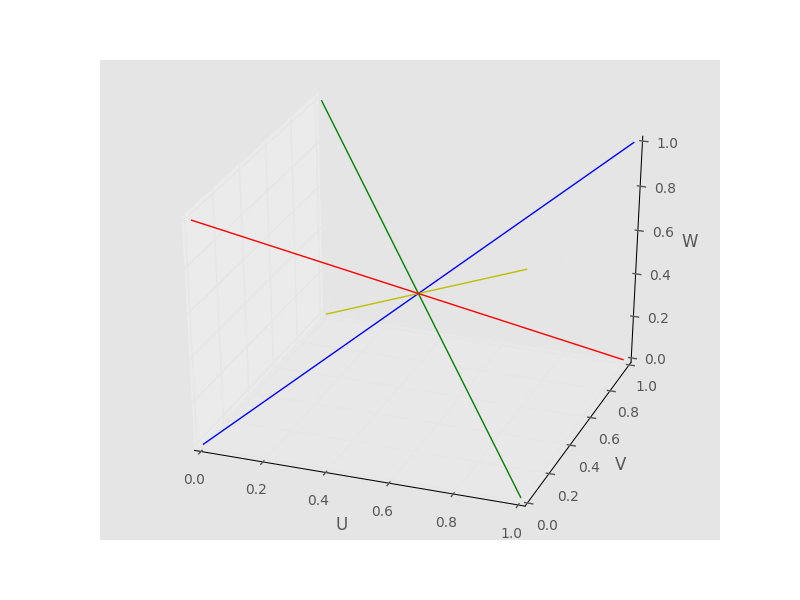
\includegraphics[width=0.7\textwidth]{Diagonals3d.png}
    \centering
    \caption{Examples of diagonals, \emph{The blue one is [(0,0,0),(1,1,1)], the yellow one is [(0,1,0),(1,0,1)], the green one is [(0,1,1),(1,0,0)],  and the red one is [(0,0,1),(1,1,0)] }}
\end{figure}

\begin{figure}
  	\centering
    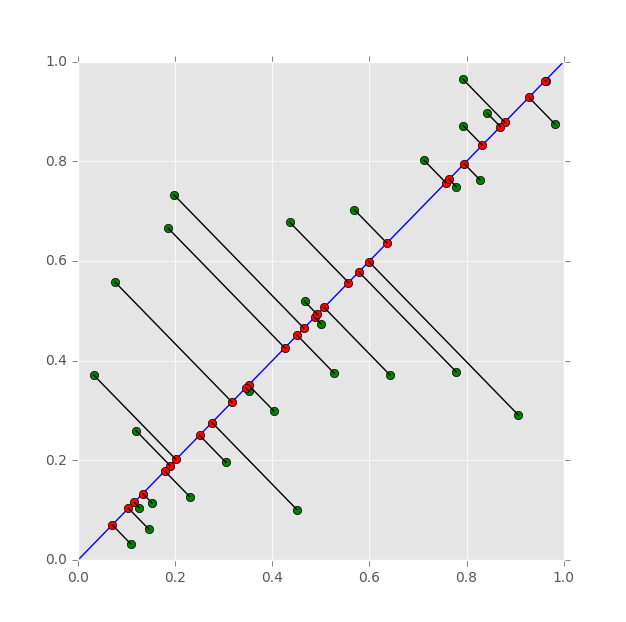
\includegraphics[width=0.7\textwidth]{proj2Ddiag0.png}
    \caption{Projection of 30 points on the [(0,0),(1,1)] diagonal \emph{The diagonal is in blue, the initial points are green and their projections are red.}}
\end{figure}

	\begin{figure}
  	\centering
    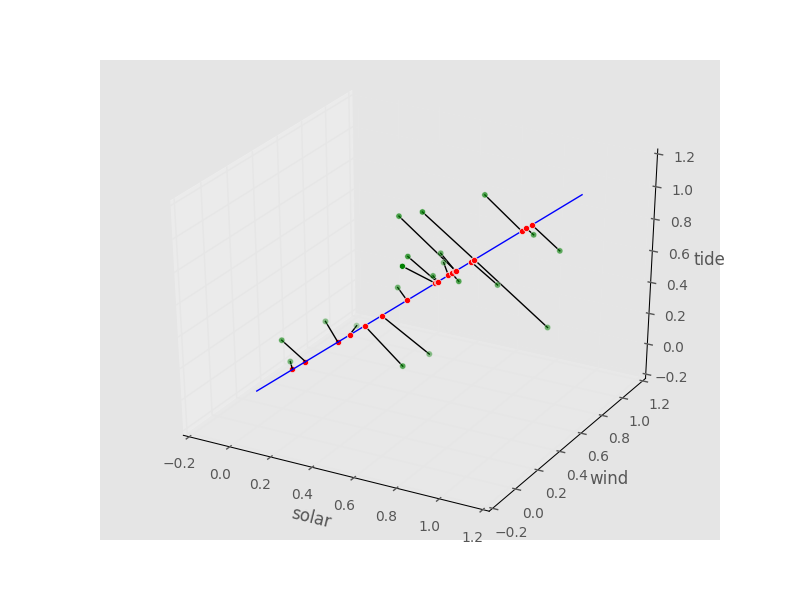
\includegraphics[width=0.7\textwidth]{proj3d.png}
    \caption{Projection of 20 points on the [(0,0,0),(1,1,1)] diagonal \emph{The diagonal is in blue, the initial points are green and their projections are red.}}
\end{figure}
	   
	  \begin{figure}
  
    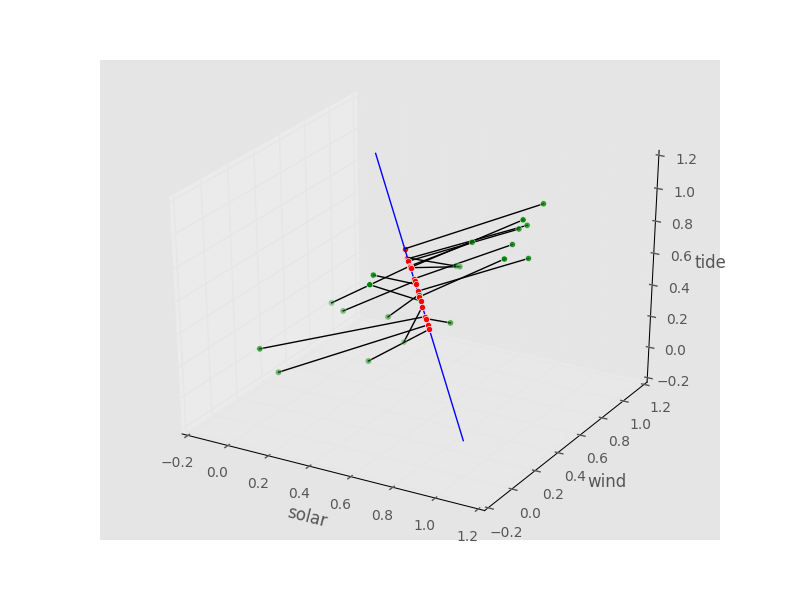
\includegraphics[width=0.7\textwidth]{proj3Ddiag2.png}
    \centering
    \caption{Projection of 20 points on the [(1,0,0),(0,1,1)] diagonal \emph{The diagonal is in blue, the initial points are green and their projections are red.}}
\end{figure}


	\subsubsection{Distribution on the diagonal}
	We now want to study the distribution of the points projected on the diagonal to compare it to a uniform distribution. Since the diagonal is a segment, each point x of the diagonal can be described by only one scalar number $\lambda$ : $x = (1-\lambda)a+\lambda b $ (cf Definition of the diagonal). \newline
	$\lambda$ can be understood as the normalised distance between a and x :
	\begin{equation*}
		\| x-a \|	= \| (1-\lambda)a+\lambda b\|
					= \lambda \| a - b \|
					= \lambda \sqrt{d} 
	\end{equation*}
Where $\| . \|$ is a norm in our space.\newline
\newline
But $\lambda$ can be easily evaluated by taking the first coordonates of x : 
	\begin{equation*}
		x_1 = (1-\lambda)a_1 + \lambda b_1 = (1-\lambda) *0 + \lambda *1 = \lambda 
	\end{equation*}
This equality is possible thanks to our useful convention $(a_1,b_1)= (0,1)$.\newline
\newline
We now have a unique number that should be uniformly distributed on [0,1].

	

	  
	  \subsection{Our algorithm}
	  
	  For each day j do :

\begin{itemize}

\item Using all day \begin{math}i \leq j-1\end{math}, fit a parametric distribution model with copula \begin{math} C_j \end{math}

\item Generate n realizations U of the random variable with the copula dependance and uniform marginals :\newline

	Generate \begin{math} \textbf{U}=(U_1,...,U_n) \end{math} with each \begin{math} U_i = (U_{i,1},...,U_{i,d}) \in [0,1]^d \end{math} \newline
\newline	
	 where \begin{math} \forall i \in \llbracket 1,n \rrbracket , \newline \mathbb{P} (U_{i,1} \leq u_1,..., U_{i,d} \leq u_d )= C(u_1,...,u_d) \text{ and } \newline
	( \forall j \in \llbracket 1,d \rrbracket, U_{i,j} \end{math} is uniformly distributed on [0,1].) \newline
	For example, n=10000  \newline
	
	
	
\item For each diagonal $\Delta$ : 
\item 
Project all the \begin{math} U_i \end{math} on the diagonal
\newline
	Define \begin{math} \textbf{V}_{\Delta} =(V_{\Delta ,1},...,V_{\Delta ,n})=(P_\Delta(U_1),...,P_\Delta(U_n)) \end{math}

\item Define the empirical distribution on this diagonal : \newline
\newline
	\begin{math} F_\Delta (X) = \frac{1}{n} \sum_{k=1}^n \mathds{1}_{V_{\Delta ,k} \leq X} \end{math}
	\newline
	\newline
	where \begin{math} a \leq b \iff \forall i \in \llbracket 1,d \rrbracket,  a_i \leq b_i  \end{math}
	
\item Observe with the data what happened on day j \newline
		Call this observation $O_j = (O_{j,1},...,O_{j,d})$

\item Pass it in the copula space \newline
		Define \begin{math} Q_j = (F_1 (O_{j,1}),...,F_d (O_{j,d})) \end{math} \newline
		where the $F_i$ are the cumulative density functions of the marginals estimated with another method.
		
\item Project $Q_j$ on the diagonal \newline
		Define $R_{\Delta ,j} = P_\Delta (Q_j)$

\item Compute its "rank" \newline Define $S_{\Delta,j} = F_\Delta (R_{\Delta,j})  $ \newline

\item Either compute the distance between the empirical distribution of the $S_{\Delta}=(S_{\Delta,i})_{i \in days}$  and the uniform distribution on [0,1].

\item Or make a histogram with the $S_{\Delta}=(S_{\Delta,i})_{i \in days}$
	\begin{math} F_\Delta^{-1} (P_j) \end{math}
	
	\subsection{Test code}
	
	In this section, I will explain how we excecuted this algorithm with different parameters. They are arguments of many test functions I wrote and are just strings defining options :\newline
	
	\texttt{source} : the type of power source we want it can be 'solar' or 'wind'\newline
	
	\texttt{datatype} : if the data are power ('actuals'), errors ('errors), a normal distributed sample ('normal-sample') or a uniformly distributed sample ('uniform-sample'), the two last ones are options to make verifications. \newline
	
	\texttt{segment\_marginals} : to segment the data to fit the marginals, you can either take only the date at the hour of your dps ('hour') or fit this marginal with the data of the whole day ('anytime'). Note : this is not the way the data are segmented to fit the copula.
	
	\texttt{kind} : which projection you want it can be on a diagonal (\texttt{"diagonal"}), a marginal (\texttt{"marginal"}) or can even compose with the kendall function (\texttt{"kendal"}). \newline
	
	\texttt{index} : the index of the diagonal or the marginal you want to project on. Diagonals are indexed in the order of diag. list of diags. Marginals are index as the coordonates. index does not matter for kendall function.\newline
	
	\texttt{method} : way you choose the data to fit the distributions, you can either fit copulas and marginals with the datas of the whole year and check the observation then ('wholeyear'), or you can decide to just use the days before the one you are computed ('daytoday')
	
\end{itemize}

\newpage

\section{Results and analysis}
I executed the experiment described previously on different sets of datas from CAISO and then from BPA. Because CAISO datasets for the years 2014 and 2015 were not big enough to be representative, I then did all my experiments with the datas from BPA from May 2012 to April 2017. All the figures presented below are obtained from the BPA datas thanks to the algorithm described above. Because I did not want to make the tests more complex, I only worked on wind power, it will nearly be the same with solar power except that I could not consider the hours during the night.

\subsection{Main experiment with actuals}

The simplest experiment we can imagine is to test if our different copulas fit well the correlation between wind power production at two adjacent hours. So I computed the algorithm of section~\ref{sec:method} with the actuals power at noon and at 1 PM. The obtained histograms are presented below.

\begin{figure}[H]
  
    \includegraphics[width=0.8\textwidth]{actuals12_13_S_diag0_univariate-empirical_hour_histogram.png}
    \centering
    \caption{Results of the test on the dependance between the actuals at 12 and 13 when projected on diagonal [(0,0),(1,1)] and without segmentation}
\end{figure}

One can see that, except for the independance copula, these histograms look very flat. (The gumbel copula is not represented on this graph for presentation issues but has also been calculated as one can see in the EMD results below). These results show that our copulas fit well highly correlated datas on the direct diagonal.


\begin{figure}[h]
\centering
\begin{tabular}{|c|c|c|c|c|}
\hline
Diagonal & Copula & (0, 1) & (0, 0.1) & (0.9, 1) \\ \hline
  
& gaussian-copula & 0.0061 & 0.0075 & 0.0065 \\ \cline{2-5} 
& student-copula & 0.0066 & 0.0073 & 0.0045 \\ \cline{2-5} 
& frank-copula & 0.0072 & 0.0079 & 0.0073 \\ \cline{2-5} 
[[0, 0], [1, 1]] & clayton-copula & 0.0064 & 0.0087 & 0.0128 \\ \cline{2-5} 
& gumbel-copula & 0.0067 & 0.0065 & 0.0058 \\ \cline{2-5}
& empirical-copula & 0.0065 & 0.0062 & 0.0069 \\ \cline{2-5} 
& independence-copula & 0.0830 & 0.0412 & 0.0449 \\ \hline 
\end{tabular}
\caption{The EMD results for wind actuals at 12 and 13 with univariate empirical marginals on diagonal [[0, 0], [1, 1]]}
\end{figure} 

When we look at the earth mover distances between the S vectors we computed and a uniformly and regularly distributed vector on [0,1] with the same length, no copula is way better than the others. Indeed, the differences between these copulas are so little that we cannot tell if those differences are simply due to the randomness of the experiment. The only exception is the independence copula which fits worse the data than all other copulas. This looks reasonable and reassuring considering this data are highly correlated. It means that using copulas is not useless.



\begin{figure}[H]
  
    \includegraphics[width=0.8\textwidth]{actuals12_13_S_diag1_univariate-empirical_hour_histogram.png}
    \centering
    \caption{Results of the test on the dependance between the actuals at 12 and 13 when projected on diagonal [(0,1),(1,0)] and without segmented the datas}
\end{figure}
When we look at the projection on the other diagonal, we see that our copulas are less precised to fit the anticorrelation. Nevertheless, they are not U-shaped or $\Lambda$-shaped, so we can assume that these imprecison is just noise due to the lack of data in the anticorrelation areas next to the corners. The method might converge slowlier on this diagonal than on the other one, so this diagonal might need more data.. When we look at the EMD results, we have the same conclusion as the direct diagonal : all copulas fits pretty well and equivalently except the independence copula which is very bad.

\begin{figure}[H]
\centering
\begin{tabular}{|c|c|c|c|c|}

\hline
Diagonal & Copula & (0, 1) & (0, 0.1) & (0.9, 1) \\ \hline
& gaussian-copula & 0.0187 & 0.0097 & 0.0113 \\ \cline{2-5}
& student-copula & 0.0275 & 0.0087 & 0.0113 \\ \cline{2-5}
 & frank-copula & 0.0184 & 0.0122 & 0.0130 \\ \cline{2-5}
[[0, 1], [1, 0]] & clayton-copula & 0.0265 & 0.0019 & 0.0032 \\ \cline{2-5}
& gumbel-copula & 0.0206 & 0.0024 & 0.0043 \\ \cline{2-5}
 & empirical-copula & 0.0144 & 0.0065 & 0.0054 \\ \cline{2-5}
 & independence-copula & 0.2090 & 0.3494 & 0.3527
\\ \hline
 
\end{tabular}
\caption{The EMD results for wind actuals at 12 and 13 with univariate empirical marginals}
\end{figure}



\subsection{Main experiment with errors}

Even if it is easier to understand power production actuals, we need to do the experiments with the errors (which is the difference forecast minus actuals) because GOSM always works with errors and its distributions are calculated using the errors and not the actuals. In order to have more precised distributions, GOSM also segments its datas which means we choose cleverly which data we will put in the arguement input\_data of our distribution class. In the case below, we segment by forecasts and with a window of 40 \%.

\begin{figure}[H]
  
    \includegraphics[width=0.8\textwidth]{errors12_13_S_diag0_univariate-empirical_hour_segmented_histogram.png}
    \centering
    \caption{Results of the test on the dependance between the errors at 12 and 13 when projected on diagonal [(0,0),(1,1)] and by segmented the datas with the forecast}
\end{figure}

\begin{figure}[H]
  
    \includegraphics[width=0.8\textwidth]{errors12_13_S_diag1_univariate-empirical_hour_segmented_histogram.png}
    \centering
    \caption{Results of the test on the dependance between the errors at 12 and 13 when projected on diagonal [(0,1),(1,0)] and by segmented the datas with the forecast}
\end{figure}

The obtained results are here similar to the results for the actuals. What we learn is that copulas are not really different for fitting the the data except for the independence copula that fits it badly as we expect.

\begin{figure}[h]
\centering
\begin{tabular}{|c|c|c|c|c|}
\hline
Diagonal & Copula & (0, 1) & (0, 0.1) & (0.9, 1) \\ \hline
 & empirical-copula &0.0168 & 0.0144 &0.0062 \\ \cline{2-5}
 & gaussian-copula & 0.0203 & 0.0189 & 0.0079 \\ \cline{2-5}
 & student-copula & 0.0178 & 0.0165 & 0.0058 \\ \cline{2-5}
[[0, 0], [1, 1]] & frank-copula & 0.0231 & 0.0265 & 0.0141 \\ \cline{2-5}
 & clayton-copula 
& 0.0242 & 0.0081 & 0.0236 \\ \cline{2-5}
 & gumbel-copula & 0.0216 & 0.0258 & 0.0036 \\ \cline{2-5}
 & independence-copula & 0.0496 & 0.0414 & 0.0364 \\ \hline
   & empirical-copula & 0.0114 & 0.0084 & 0.0043 \\ \cline{2-5}
& gaussian-copula & 0.0418 & 0.0095 & 0.0130 \\\cline{2-5}
& student-copula & 0.0311 & 0.0064 & 0.0091 \\\cline{2-5}
[[0, 1], [1, 0]]& frank-copula & 0.0463 & 0.0074 & 0.0102 \\ \cline{2-5}
& clayton-copula & 0.0397 & 0.0088 & 0.0084 \\\cline{2-5}
& gumbel-copula & 0.0400 & 0.0074 & 0.0098 \\ \cline{2-5}
& independence-copula & 0.1053 & 0.0764 & 0.0769\\ \hline
 
\end{tabular}
\caption{The EMD results for wind errors at 12 and 13 with univariate empirical marginals}
\end{figure}


\subsection{Verification and marginals}

In order to verify if our method was working, I coded different other tools linked to the tests. I first needed to clean the datas so that the software won't fail. I suppressed all the datas that had no sense such as strings instead of float and converted it to \texttt{NaN}. Then each time I would call a a new distribution object, I would drop the \texttt{NaN} in the columns i am using. I also delt with the problem of datetime objects. Because I was studying the dependence between data at different hours, I wanted that the dates keep being the indexes of my dataframe and the hours become the columns while keeping the different datatypes.

Then, I needed to verify if the experiment was working with data for which we know the properties. So, I added to my dataframe, random samples that I generated with python \texttt{numpy.random} functions. All these work on data made by in the function \texttt{creates\_data} of copula.py.

\begin{figure}[H]
 \centering
    \includegraphics[width=0.8\textwidth]{datas_BPA_all_histogram_univariate-epispline.png}
    \centering
    \caption{Histograms of our data and their fitted univariate epispline pdf}
\end{figure}

I coded functions that draw plots to understand our data more. \texttt{csv\_to\_histogram} permits to draw an histogram from a dataframe stored in a csv. One can then easily see the distribution of actuals, errors to one hour forecast (EH1) or to verify if our random samples have the good properties.

I also had to check if the marginals fitted the data well, otherwise 
the whole experiment on copulas was useless. That is why I added the possibility to project on a marginal instead of a diagonal in the big code. In a simplier way, I added the possibility in \texttt{csv\_to\_histogram} to draw the pdf of a fitted univariate distribution of any class of the user's choice. I found that in some cases, the univariate epispline distribution can fit badly the datas. For example, it was not able to model the high probability to have a production of 0 MW. This caused me a lot of trouble for my experiments because univariate epispline were the default distribution in GOSM. But we finally decided to work with the univariate empirical distribution in our tests to temporarly avoid this problem and focus on copulas. All the experiments presented above are then computed with univariate empirical marginals.

\begin{figure}[H]  
    \includegraphics[width=0.7\textwidth]{histograms_of_errors2d.png}
    \centering
    \caption{Histograms of errors}
\end{figure}

As well as we verified our data and the fitted distribution linked with them in one dimension, I coded a function called \texttt{print\_contours} that draw a 2d histograms of our data thanks to a color code and the contours of the pdf of the fitted multivariate distribution with copula and marginals of the user choice. It also permits to compare visually if the copula seems to fit well the data. In our case, the contours plots are coherent with the datas histograms for all copula except for the independence one.

\begin{figure}[H]
    \includegraphics[width=0.6\textwidth]{pdf_contours_gaussian-copula_univariate-epispline.png}
    \centering
    \caption{Contours of the error-fitted multivariate distribution, with gaussian copula and univariate epispline marginal, pdf}
\end{figure}

%\begin{figure}
  
    %\includegraphics[width=0.7\textwidth]{pdf_contours_gumbel-copula_univariate-epispline.png}
    %\centering
    %\caption{Contours of the fitted gumbel copula pdf}
%\end{figure}



\newpage

\vspace*{\stretch{1}}

\section*{Conclusion}
\addcontentsline{toc}{section}{Conclusion}

	
	I coded a complex tool which is a small part of a larger project. With my experiments, I was able to confirm that copulas are really useful to model the dependence between our different data. We now know that all copulas fit the data that we tested with roughly the same accuracy except the independence one. However, my work consisted in the first experiments focused on specific datas. So it needs to be continued to have a larger vision of the problem and more precise conclusions with higher degrees of likelihood. But the main code is now written and permits much more experiences than the simplest ones. I give ideas of directions for future work in appendix~\ref{sec:directions}. All this code will be very useful in GOSM, every user can now choose which copula he wants and creates more precise scenario and especially more precise probability. With these more relevant inputs, a GOSM user can now run the stochastic optimization problem and test if adding copulas give better results.
	 
	Concerning this internship, I found really interesting to build a coherent and complex structure such as this distribution and copula code. I realized the importance of verifying of the procedure which can become completely wrong even if we have made a small mistake. Once the code is running, it can look like a black box which gives results we have to believe. We should always avoid that and prefer to have a precised vision of our data and our algorithmn so that we really understand what happens so we would be able to interpret correctly the results. That is why I coded many unittests which are really good verifications on the one hand and which make us understand more precisely our problem on the other hand. I also learned that dealing with real data is way more complex than simulated ones. You have many small bugs you need to fix and you do not know many things about this data. This is why I added the possibility to check and compare with simulated samples which are very easy to deal with.
	
	I enjoyed doing some research. Dealing with interesting and clever mathematical problems always insterested me. I also liked the idea that this project is useful in the field of energy. Since I am interesting in both optimization and energy, I would like to continue working on such projects. They are not closed fields since my internship was eventually more about statistics and probability theory than optimization even if it was a part of a bigger stochastic optimization problem. As I did in this internship, I would like to still be opened and also learn from other subjects. Next year, I will study a master in Universit\'e Pierre et Marie Curie in Paris to continue learning about optimization while integrating the Corps des Ing\'enieurs des Ponts Eaux et For\^ets to work on energy. My goal is to make a thesis in optimization applied to the energy and the smart grids field. This internship was a first experience for me that taught me a lot.

	\vspace*{\stretch{1}}


\newpage
\begin{thebibliography}{9}

	\bibitem{archimedeancopulas}
  	Alexander J. McNeil, Johanna Neslehova
 	 \emph{Multivariate Archimedean Copulas, d-monotone Functions and l1-norm Symmetric Distributions},Ann. Stat., 37:3059-3097, 2009.	

	\bibitem{vineconstruction}
  	Kjersti Aas, Claudia Czado, Arnoldo Frigessi, Henrik Bakken,
 	 \emph{Pair-copula construction of multiple dependence},
  	2007.
  	
  	\bibitem{fourcopulas}
  	Kjersti Aas,
 	 \emph{Modeling the dependance structure of financial assets : A survey of four copulas}
  	2004.
  	
  	\bibitem{kendallfunction}
  	Johanna F. Ziegel, Tilmann Gneiting, 
 	 \emph{Copula Calibration}, Electronic Journal of Statistics,
  	2014.
  	
  	\bibitem{ellipticalcopula}
  	Johan Segers, 
 	 \emph{Copulas: An Introduction
Part II: Models}, Columbia University, New York City,
  	9\_11 Oct 2013.

	\bibitem{prescientmethod}
  	Sabrina Nitsche, Scott Winner, C/'esar A. Silva-Monroy, Andrea Staid, Jean-Paul Watson, David L. Woodruff
 	 \emph{Improving Wind Power Prediction Intervals Using
Vendor-Supplied Probabilistic Forecast Information}.	
	
	\bibitem{hamill2000}
  	Thomas M. Hamill,
 	 \emph{Interpretation of Rank Histograms for Verifying Ensemble Forecasts},
  	2000.  	
  	
  	\bibitem{gaubert}
  	Stéphane Gaubert, Frédéric Bonnans,
  	\emph{Recherche opérationnelle : aspects mathématiques et applications},
  	Editions de l'École polytechnique,
  	2016	

	\bibitem{epispline}
	Johannes O.Royset, Roger J-B Wets,
	\emph{Nonparametric Density Estimation via Exponential Epi-Splines: Fusion of Soft and Hard Information}, 2013.	
	
	\end{thebibliography}

	\newpage
	\section*{Appendix}
	\appendix
	\section{List of files and classes}
	\label{sec:list}	 
	 
	 
	 
	 \textbf{base\_distribution.py}\newline
	 \texttt{BaseDistribution} \newline
	 \texttt{MultiDistr}
	
	 
	 \textbf{distributions.py}
	 \newline
	 \texttt{UnivariateBasicEmpiricalDistribution} \newline
	 \texttt{UnivariateEmpiricalDistribution} \newline
	 \texttt{UnivariateEpiSplineDistribution} \newline
	 \texttt{UnivariateUniformDistribution} \newline
	 \texttt{UnivariateNormalDistribution} \newline
	 \texttt{UnivariateStudentDistribution} \newline
	 \texttt{MultiNormalDistribution} \newline
	 \texttt{MultiStudentDistribution} \newline
	 
	
	 \textbf{copula.py}
	 \newline
	 \texttt{CopulaBase} \newline
	 \texttt{GaussianCopula} \newline
	 \texttt{StudentCopula} \newline
	 \texttt{FrankCopula} \newline
	 \texttt{ClaytonCopula} \newline
	 \texttt{GumbelCopula} \newline
	 \texttt{WeigthedCombinedCopula} \newline
	 \texttt{IndependenceCopula} \newline
	 \texttt{EmpiricalCopula} \newline
	 
	 \textbf{vine.py}
	\newline
	 \texttt{CVineCopula} \newline
	 \texttt{DVineCopula}\newline
	 
	\textbf{distribution\_factory.py}\newline
	 
	
	 
	 \textbf{tester.py}
	\newline
	 \texttt{MultiNormalDistributionTester} \newline
	 \texttt{UnivariateNormalDistributionTester} \newline
	 \texttt{MultiStudentDistributionTester} \newline
	 \texttt{UnivariateStudentDistributionTester}\newline
	 \texttt{CopulaTester} \newline
	 \texttt{VineCopulaTester}
	 
	 
 	\newpage
	
	\section{Distribution formulas}
	\label{sec:distributions}
	 \texttt{UnivariateBasicEmpiricalDistribution} is the simplest distribution you can build without making an hypothesis on the model. It assumes that all the results in the \texttt{input\_data} are the only possible ones and that they are equiprobable. This gives us a method to generate a sample, we simply pick randomly one element of \texttt{input\_data}. If we note $Y = (Y_1,...,Y_n) = \texttt{input\_data}$, the functions would be :
	\begin{equation*}
  	F(x) = \frac{1}{n}\sum_{k=1}^n \mathds{1}_{Y_k\leq x}
  	\end{equation*}
  	\begin{equation*}
  	\mathbb{P}(X=x) = \frac{1}{n}\sum_{k=1}^n \mathds{1}_{Y_k = x}
  	\end{equation*}
  	One can notice that F is not continuous, that implies that f is not well defined. \newline
	 
	 \texttt{UnivariateEmpiricalDistribution} works almost like \texttt{UnivariateBasicEmpirical} but avoids the problem of continuity by cleverly interpolating lines between the points we have. When the set of data is big enough it gives the same result than \texttt{UnivariateBasicEmpricalDistribution}. \newline
	 
	 \texttt{UnivariateEpiSplineDistribution} is a more clever object obtained thanks to the resolution of an optimization problem where the cdf as a particular shape (for more information see \cite{epispline}) : \newline
	 \begin{equation*}
  	F(x) = e^{-g(x)}\text{, where }g\text{ is polynomial by pieces}
  	\end{equation*}
  	To use this class, it needs a \texttt{gosm\_options} object to be defined "globally". For example, one can choose the number N which indicates how much subsegments we want to divide our initial segment to create each piece of the polynomial function. Plus, this class needs the installation of the language pyomo and of the solver ipopt. To learn more about these installation, check \texttt{GOSM} user manual. This class is unusual because it was extracted from an earlier version of software called \texttt{Prescient}.\newline
  	
	 
	 \texttt{UnivariateUniformDistribution} contains only two parameters called \texttt{a} and \texttt{b} who represent respectively the minimum and the maximum of the distribution. When an object of this class is called with \texttt{input\_data}, the \texttt{\_\_init\_\_} method, assign the minimum of \texttt{input\_data} to $a$ and its maximum to $b$.
	 \begin{equation*}
	 a = \texttt{a} = \texttt{min(input\_data)}
	 \end{equation*}
	 \begin{equation*}
	 b = \texttt{b}= \texttt{max(input\_data)}
	 \end{equation*}
	 \[
   		f(x) =
   		\begin{cases}
        
    	\frac{1}{b-a} & \quad \text{if } x \in [a,b]\\
    	0  & \quad \text{else}\\
  \end{cases}
  \]
	 \[
   		F(x) =
   		\begin{cases}
        0  & \quad \text{if } x \leq a \\
    	1 & \quad \text{if } x \geq b \\
    	\frac{x-a}{b-a} & \quad \text{else}
  \end{cases}
  \]
  
  \texttt{UnivariateNormalDistribution} has two parameters \texttt{mean} and \texttt{var} which are stored as attributes. We present below the main formulas that define this class. Each time we represent parameters with their names in the python code and with its usual mathematical notation so that the formulas are not too hard to read.
  	\begin{equation*}
  	\mu = \texttt{mean} =  \texttt{mean(input\_data})
  	\end{equation*}
  	\begin{equation*}
  	\sigma^2 = \texttt{var} = \texttt{var(input\_data})
  	\end{equation*}
  	\begin{equation*}
  	f(x) = \frac{1}{\sqrt{2\pi \sigma^2}}e^{-\frac{(x-\mu)^2}{\sigma^2}}
  	\end{equation*}
  	\begin{equation*}
  	F(x) = \int_{-\infty}^x \frac{1}{\sqrt{2\pi\sigma^2}}e^{-\frac{(y-\mu)^2}{\sigma^2}}dy
  	\end{equation*}
  	
  	\texttt{UnivariateStudentDistribution}
  	
  	\begin{equation*}
  	\mu = \texttt{mean} = \texttt{mean(input\_data)}
  	\end{equation*}
  	\begin{equation*}
  	\nu = \texttt{df} = \texttt{2var(input\_data)/(var(input\_data)-1)}
  	\end{equation*}
  	\begin{equation*}
  	f(x) = \frac{1}{\sqrt{\nu\pi}}\frac{\Gamma(\frac{\nu+1}{2})}{\Gamma(\frac{\nu}{2})}\left(1+\frac{(x-\mu)^2}{\nu}\right)^{-\frac{\nu+1}{2}}
  	\end{equation*}
  	\begin{equation*}
  	F(x) = \int_{-\infty}^x \frac{1}{\sqrt{\nu\pi}}\frac{\Gamma(\frac{\nu+1}{2})}{\Gamma(\frac{\nu}{2})}\left(1+\frac{(y-\mu)^2}{\nu}\right)^{-\frac{\nu+1}{2}}dy
  	\end{equation*}
	 
	 
	 \texttt{MultiNormalDistribution}
	 
  	\begin{equation*}
  	\mu = \texttt{mean} = \texttt{mean(input\_data)}
  	\end{equation*}
  	\begin{equation*}
  	K = \texttt{cov} = \texttt{cov(input\_data)}
  	\end{equation*}
  	\begin{equation*}
  	f(x) = \frac{1}{(2\pi)^{\frac{d}{2}}\sqrt{det(K)}}e^{-\frac{(x-\mu)^\top K^{-1} (x-\mu)x}{2}}
  	\end{equation*}
  	\begin{equation*}
  	F(x) = \int_{-\infty}^x \frac{1}{(2\pi)^{\frac{d}{2}}\sqrt{det(K)}}e^{-\frac{(y-\mu)^\top K^{-1} (y-\mu)}{2}}dy
  	\end{equation*}
  	
  	\texttt{MultiStudentDistribution}
  	
  	\begin{equation*}
  	\mu = \texttt{mean} = \texttt{mean(input\_data)}
  	\end{equation*}
  	\begin{equation*}
  	\nu = \texttt{df}
  	\end{equation*}
  	\begin{equation*}
  	K = \texttt{cov} = \texttt{cov(input\_data)}
  	\end{equation*}
  	\begin{equation*}
  	f(x) = \frac{\Gamma (\frac{\nu +d}{2})}{\Gamma
	 (\frac{\nu}{2})(\nu \pi)^{\frac{d}{2}}\sqrt{det(K)}}\left(1+\frac{1}{\nu}(x-\mu)^\top K^{-1} (x-\mu) \right)^{-\frac{\nu +d}{2}}
  	\end{equation*}
  	\begin{equation*}
  	F(x) = \int_{-\infty}^x \frac{1}{\sqrt{\nu\pi}}\frac{\Gamma(\frac{\nu+1}{2})}{\Gamma(\frac{\nu}{2})}\left(1+\frac{(y-\mu)^2}{\nu}\right)^{-\frac{\nu+1}{2}}dy
  	\end{equation*}
	
	\section{Copula formulas}
	\label{sec:copulas}	
	\subsection{Elliptical copulas}
	\subsubsection{Gaussian Copula}
	
\begin{math} \mathcal{N}(x)=\frac{1}{\sqrt{2\pi}}\int_{-\infty}^{x} e^{-\frac{t^{2}}{2}}dt \end{math}
	
	\paragraph{C function in dimension d}
	
	
	\begin{math}
	 C_{K}(u_{1},...u_{d})= \mathlarger{ \int_{-\infty}^{\mathcal{N}^{-1}(u_{1})}...\int_{-\infty}^{\mathcal{N}^{-1}(u_{d})} \frac{1}{(2\pi)^{\frac{d}{2}}\sqrt{det(K)}}e^{-\frac{x^\top K^{-1} x}{2}}dx}
	\end{math}
	\newline
	\newline
	With a change of variable, we have also \newline
	\newline
	\begin{math}
	C_{K}(u_{1},...u_{d})=  \mathlarger{ \int_{0}^{u_{1}}...\int_{0}^{u_{d}} \frac{1}{\sqrt{det(K)}}e^{-\frac{\mathcal{N}^{-1}(x)^\top (K^{-1}-I_{d}) \mathcal{N}^{-1}(x)}{2}}dx}
	\end{math}
	\newline
	\newline
	\newline
	where \begin{math} \mathcal{N}^{-1}(x) =  \begin{pmatrix}
   \mathcal{N}^{-1}(x_{1}) \\
  \vdots   \\
   \mathcal{N}^{-1}(x_{d})  
 \end{pmatrix}\end{math}
 
\paragraph{C function in dimension 2} 
 	
 	In dimension 2, all matrix of correlation can be written \begin{math} K = 
 \begin{pmatrix}
  1 & \rho \\
  \rho & 1
 \end{pmatrix}
\end{math}. So we will only consider one parameter \begin{math} \rho \end{math}.\newline
\newline

\begin{math}
	C_{\rho} (u,v) = \mathlarger{\int_{-\infty}^{\mathcal{N}^{-1}(u)}\int_{-\infty}^{\mathcal{N}^{-1}(v)} \frac{1}{2\pi\sqrt{1-\rho^{2}}}e^{-\frac{x^2-2\rho x y +y^{2}}{2(1-\rho^{2})} }dx dy} 
\end{math}
\newline
\newline
With the same change of variable, we have also
\newline
\begin{math}
	C_{\rho} (u,v) = \mathlarger{\int_{0}^{u}\int_{0}^{v} \frac{1}{\sqrt{1-\rho^{2}}}e^{-\frac{\rho^{2}\mathcal{N}^{-1}(x)^2-2\rho\mathcal{N}^{-1}(x)\mathcal{N}^{-1}(y) + \rho^{2} \mathcal{N}^{-1}(y)^{2}}{2(1-\rho^{2})} }dx dy} 
\end{math} 
 

	\paragraph{c function in dimension n}
	\begin{equation*}
	c_{K}(u_1,...,u_d)=\frac{1}{\sqrt{det(K)}}e^{-\frac{\mathcal{N}^{-1}(u)^\top (K^{-1}-I_{d}) \mathcal{N}^{-1}(u)}{2}}
	\end{equation*}

	where \begin{math} \mathcal{N}^{-1}(u) =  \begin{pmatrix}
   \mathcal{N}^{-1}(u_{1}) \\
  \vdots   \\
   \mathcal{N}^{-1}(u_{d})  
 \end{pmatrix}\end{math}



	\subsubsection{Student Copula}
	 We will note \begin{math} t_\nu(x)=\frac{\Gamma (\frac{\nu+1}{2})}{\sqrt{\nu \pi} \Gamma (\frac{\nu}{2})}\int_{-\infty}^{x} \left(1+\frac{t^2}{\nu}\right)^{-\frac{\nu +1}{2}}dt \end{math}, the cumulative density function of the student distribution with degree of freedom \begin{math} \nu \end{math} and \begin{math}  t_\nu^{-1} \end{math} its inverse. \newline
	We could write both with the regularized incomplete Beta function \newline \begin{math} I_{a,b}(x) = \frac{1}{B(a,b)} \int_{0}^{x} t^{a-1}(1-t)^{b-1}dt \newline = \frac{\Gamma (a+b)}{\Gamma (a)\Gamma (b)} \int_{0}^{x} t^{a-1}(1-t)^{b-1}dt\end{math} \newline
	\newline
	and its inverse \begin{math} I_{a,b}^{-1} \end{math} : \newline
	\[
   		t_\nu (x) =  \begin{cases}
        I_{\frac{\nu}{2},\frac{1}{2}}(\frac{\nu}{x^2+\nu})  & \quad \text{if } x \leq 0 \\
    	1-I_{\frac{\nu}{2},\frac{1}{2}}(\frac{\nu}{x^2+\nu}) & \quad \text{if } x \geq 0\\
  	\end{cases}
  	\]
  	
  	and \newline
  	\[
   		t_\nu^{-1} (x) =  \begin{cases}
        -\sqrt{\nu (\frac{1}{I^{-1}_{\frac{\nu}{2},\frac{1}{2}}(2y)}-1)}  & \quad \text{if } x \leq \frac{1}{2} \\
    	\sqrt{\nu (\frac{1}{I^{-1}_{\frac{\nu}{2},\frac{1}{2}}(2(1-y))}-1)}  & \quad \text{if } x \geq \frac{1}{2}\\
  	\end{cases}
  	\]

	\paragraph{Generate X}
	To generates our U vector in the $[0,1]^d$ space, we need to first generates a X vector in the $\mathbb{R}^d$ space following a Multivariate Student Distribution. Thus, we use the equality in law :
	\begin{equation*}
	\sqrt{\frac{\nu}{S}} Z \sim t_\nu (0,K)
	\end{equation*}
	where $s \sim \chi_\nu^2$ and $Z \sim \mathcal{N} (0,K)$
	
	\paragraph{C function in dimension d}
	
	
	\begin{equation*}
	 C_{K}(u_{1},...u_{d})= \mathlarger{ \int_{-\infty}^{t_\nu^{-1}(u_{1})}...\int_{-\infty}^{t_\nu^{-1}(u_{d})} \frac{\Gamma (\frac{\nu +d}{2})}{\Gamma
	 (\frac{\nu}{2})(\nu \pi)^{\frac{d}{2}}\sqrt{det(K)}}\left(1+\frac{1}{\nu}x^\top K^{-1} x \right)^{-\frac{\nu +d}{2}}dx}
	\end{equation*}
	\newline
	\newline
	With a change of variable, we have also \newline
	\newline
	\begin{math}
	C_{K}(u_{1},...u_{d})=  \mathlarger{ \int_{0}^{u_{1}}...\int_{0}^{u_{d}} \frac{\Gamma (\frac{\nu +d}{2}) \Gamma (\frac{\nu}{2})^{^{d-1}}}{\sqrt{det(K)}\Gamma (\frac{\nu +1}{2})^{^{d}}\Pi_{j=1}^d 1+\frac{t_\nu^{-1}(x_j)^2}{2})^{-\frac{\nu+1}{2}}}\left(1+\frac{1}{\nu}t_\nu^{-1}(x)^\top K^{-1} t_\nu^{-1}(x) \right)^{-\frac{\nu +d}{2}}dx}
	\end{math}
	\newline
	\newline
	\newline
	where \begin{math} t_\nu^{-1}(x) =  \begin{pmatrix}
   t_\nu^{-1}(x_{1}) \\
  \vdots   \\
   t_\nu^{-1}(x_{d})  
 \end{pmatrix}\end{math}
 
\paragraph{C function in dimension 2} 
 	
 	In dimension 2, all matrix of correlation can be written \begin{math} K = 
 \begin{pmatrix}
  1 & \rho \\
  \rho & 1
 \end{pmatrix}
\end{math}. So we will only consider one parameter \begin{math} \rho \end{math}.\newline
\newline

\begin{math}
	C_{\rho,\nu} (u,v) = \mathlarger{\int_{-\infty}^{t_\nu^{-1}(u)}\int_{-\infty}^{t_\nu^{-1}(v)} \frac{1}{2\pi\sqrt{1-\rho^{2}}}\left(1+\frac{x^2 -\rho x y + y^2}{\nu (1-\rho^2)}\right)^{-\frac{\nu +2}{2}}dx dy} 
\end{math}
\newline

 
\paragraph{Partial derivative of C}


If we derivate the formula above, we obtain (cf Pair copula constructions of muliple dependance) : \newline
\begin{math}
h(u,v,\rho,\nu)=\frac{\partial C_{\rho,\nu}}{\partial v} (u,v) = t_\nu \bigg(\frac{t_\nu^{-1}(u)-\rho t_\nu^{-1}(v)}{\sqrt{\frac{(\nu+t_\nu^{-1}(v)^2)(1-\rho ^2)}{\nu+1}}}\bigg)
\end{math}

If we inverse this function, we obtain\newline
\newline
\begin{math}
h^{-1}(u,v,\rho,\nu) = t_\nu (\sqrt{\frac{(\nu+t_\nu^{-1}(v)^2)(1-\rho)}{\nu+1}}t_\nu^{-1}(u)+\rho t_\nu^{-1}(v))
\end{math}

	 
	\paragraph{c function in dimension d}	 
	
	\begin{equation*}	 
	 c_{K,\nu} (u_{1},...,u_{d}) = \frac{\Gamma (\frac{\nu +d}{2}) \Gamma (\frac{\nu}{2})^{^{d-1}}}{\sqrt{det(K)}\Gamma (\frac{\nu +1}{2})^{^{d}}\Pi_{j=1}^d (1+\frac{t_\nu^{-1}(u_{j})^2}{2})^{-\frac{\nu+1}{2}}}\left(1+\frac{1}{\nu}t_\nu^{-1}(u)^\top K^{-1} t_\nu^{-1}(u) \right)^{-\frac{\nu +d}{2}}
	\end{equation*}
	\newline
	 where \begin{math} t_\nu^{-1}(u) =  \begin{pmatrix}
   t_\nu^{-1}(u_{1}) \\
  \vdots   \\
   t_\nu^{-1}(u_{d})  
 \end{pmatrix}\end{math}

	 

\subsection{Archimedean Copulas}
   Archimedean copulas take the form :
   \newline
   \newline
   \begin{math}
   C(u_{1},...,u_{d})= \Phi(\Phi^{-1}(u_{1})+...+\Phi^{-1}(u_{d}))
   \end{math}
   \newline
   \newline
   where \begin{math} \Phi \end{math} is the Laplace transform of a positive nonzero random variable Y :
	\begin{math} \Phi (u)=\mathbb{E}(e^{-uY})
	\newline
	\newline
	\Phi \end{math} is called the generator function.
	\newline
	It generally depends on a parameter called \begin{math} \theta \end{math}.
	\newline
	In some papers, the definition of the generator function and its inverse can be inverted. We will use the definition above which gives us simpler formulas.
	\newline
	
	
	All of the next formulas can be expressed with the generator function.\newline
	For example, if we refer to \cite{archimedeancopulas}, we can write the Kendall distribution function thanks to the generator function :
	\[
   		\mathcal{K}_C (x) =
   		\begin{cases}
        \frac{(-1)^{d-1}(\Phi^{-1}(0))^{d-1}}{(d-1)!}\Phi_-^{(d-1)}(\Phi^{-1}(0))  & \quad \text{if } x=0 \\
    \sum\limits_{k=0}^{d-2}\frac{(-1)^{k}(\Phi^{-1}(x))^{k}\Phi^{(k)}(\Phi^{-1}(x))}{k!}+\frac{(-1)^{d-1}(\Phi^{-1}(x))^{d-1}\Phi_-^{(d-1)}(\Phi^{-1}(x))}{(d-1)!} & \quad \text{if } x \in ]0,1] \\
  \end{cases}
  \]
   	\subsubsection{Frank Copula}
   	\paragraph{Generator, generator inverse and derivatives}
   	\begin{math}
   		\theta \in \mathbb{R} \backslash \{ 0 \} \newline
   		\newline
   		\Phi_{\theta}(t)= -\frac{1}{\theta}log(1+e^{-t}(e^{-\theta}-1))
   		\newline
   		\newline
   		\Phi_{\theta}^{-1}(t)=-log(\frac{e^{-\theta t}-1}{e^{-\theta}-1}) 
   		\newline
   		\newline
   		\Phi_{\theta}^\prime (t)= \frac{e^{-t}}{\theta (\frac{1}{e^{-\theta} -1}+e^{-t})}
   		\newline
   		\newline
   		\Phi_{\theta}^{\prime \prime} (t)= \frac{-e^{-t}}{\theta (e^{-\theta} -1) (\frac{1}{e^{-\theta} -1}+e^{-t})^2}
   	\end{math}
   	
   	
   	\paragraph{C function in dimension 2}
   	\begin{math}
   		C_{\theta}(u,v) = -\frac{1}{\theta}log(1+\frac{(e^{\theta u}-1)(e^{\theta v}-1)}{e^{-\theta}-1})
   	\end{math}
   	
   	\paragraph{Partial derivative of C and inverse}
   	\begin{math}
   		h(u,v,\theta)=\frac{\partial C_{\theta}}{\partial v} (u,v) = \frac{e^{\theta u}-1}{e^{\theta u}+e^{\theta v}-e^{\theta (u+v-1)}-1}
   	\newline
	\newline
	\text{We first solve } \frac{a X + b}{c X + d}=y \text{, where } a = 1, b =-1, c= 1-e^{\theta (v-1)}, d = e^{\theta v}-1\newline
	\newline
	\text{We have then } X = \frac{dy-b}{a-cy}\newline
	\newline
	\text{We solve } e^{\theta u}=X : u = \frac{1}{\theta}log(X)\newline
	\newline
	\text{So, we now have}\newline
  	h^{-1}(u,v,\theta) = \frac{1}{\theta}log(\frac{(e^{\theta v}-1)u+1}{1-(1-e^{\theta (v-1)})u})
   	\end{math}
   	
   	\paragraph{c function in dimension 2}
   	
   	\begin{math}
   	c_\theta (u,v) = \frac{\theta e^{\theta (u+v)} (1-e^{-\theta})}{(e^{\theta u}+e^{\theta v}-e^{\theta (u+v-1)}-1)^2}
   	\end{math}
   	
   	
   	\subsubsection{Gumbel Copula}
   	\paragraph{Generator and generator inverse}
   	\begin{math}
   		\theta \in  [1,\infty[ \newline
   		\newline
   		\Phi_{\theta}(t)= e^{-t^{ \frac{1}{\theta} }}
   		\newline
   		\Phi_{\theta}^{-1}(t)=(-log(t))^{\theta} \newline
   		\Phi_{\theta}^\prime (t) = -\frac{1}{\theta} t^{ \frac{1-\theta}{\theta}} e^{-t^{ \frac{1}{\theta} }} \newline
   		\Phi_{\theta}^{\prime \prime} (t) = ((-\frac{1}{\theta} t^{ \frac{1-\theta}{\theta}})^2 - \frac{1-\theta}{\theta^2} t^{ \frac{1-2\theta}{\theta}}) e^{-t^{ \frac{1}{\theta} }}
   	\end{math}
   	\paragraph{C function in dimension 2}
   	\begin{math}
   		C_{\theta}(u,v) = e^{-((-log(u))^{\theta}+(-log(v))^{\theta})^{\frac{1}{\theta}}}
   	\end{math}
   	\paragraph{Partial derivative of C and inverse}
   	\begin{math}
   		h(u,v,\theta)=\frac{\partial C_{\theta}}{\partial v} (u,v) = \frac{1}{v}(-log(v))^{\theta-1}((-log(u))^{\theta}+(-log(v))^{\theta})^{\frac{1}{\theta}-1}e^{-((-log(u)^{\theta}+(-log(v))^{\theta})^{\frac{1}{\theta}}}
	\newline
	\newline
	\text{We have to introduce the lambert W function which is the inverse of } x \to x e^{x} :\newline
	W(x)e^{W(x)}=x
	\newline\newline
	\text{For } x \geq 0, ye^{y}= x \text{ has only one solution y.}\newline
	\text{So, there is no ambiguity to define } W(x) \text{ if } x\geq 0.
	\newline
	\newline
	\text{We first solve } \lambda X^\alpha e^{-X} = y \text{ where } \lambda = \frac{(-log(v))^{\theta-1}}{v}, \alpha = 1-\theta
	\newline
	\newline
	\text{We obtain } X = \alpha W(\frac{1}{\alpha}(\frac{y}{\lambda})^{\frac{-1}{\theta-1}})
	\newline
	\newline
	\text{Then, we solve } X = ((-log(u))^{\theta}+(-log(v))^{\theta})^{\frac{1}{\theta}}
	\newline
	\newline
	\text{which gives us } u = e^{-(X^{\theta}-(-log(v))^{\theta})^{\frac{1}{\theta}}}
	\newline
	\newline
	\text{Finally, we have }
  	h^{-1}(u,v,\theta) = e^{-(((\theta-1)W(\frac{-log(v)}{\theta-1}(vu)^{\frac{-1}{\theta -1}}))^{\theta}-(-log(v))^{\theta})^{\frac{1}{\theta}}}
	\end{math}
   	
	\paragraph{c function in dimension 2}
	
	\begin{math}
		c_\theta (u,v) =  \frac{C_\theta (u,v)}{u v} ((-log(u)^{\theta}+(-log(v))^{\theta})^{-2+\frac{2}{\theta}} [1+ (\theta -1)((-log(u)^{\theta}+(-log(v))^{\theta})^{-\frac{1}{\theta}}]
	\end{math}   	
   	
   	
   	
   	\subsubsection{Clayton Copula}	
   \paragraph{Generator, generator inverse and derivatives}
   	\begin{math}
   		\theta \in  [-1,\infty[ \backslash \{ 0 \} \newline
   		\newline
   		\Phi_{\theta}(t)= (1+\theta t)_+^{-\frac{1}{\theta} }
   		\newline
   		\Phi_{\theta}^{-1}(t)=\frac{1}{\theta}(t^{-\theta}-1) \newline
   		\newline
   		\Phi_{\theta}^{(n)}(t) = (-1)^n (1+\theta t)^{-\frac{1+n \theta}{\theta}} \prod\limits_{k=0}^{n-1} (1 + k \theta)
   	\end{math}
   	
	\paragraph{C function in dimension 2}
   	\begin{math}
   		C_{\theta}(u,v) = (max\{u^{-\theta}+v^{-\theta}-1;0\})^{-\frac{1}{\theta}}
   	\end{math}
	\paragraph{Partial derivative of C and inverse}
   	\[
   		h(u,v,\theta)=\frac{\partial C_{\theta}}{\partial v} (u,v) = \begin{cases}
        v^{-\theta-1}(u^{-\theta}+v^{-\theta}-1)^{-\frac{1}{\theta}-1}  & \quad \text{if } u^{-\theta}+v^{-\theta} \geq 1 \\
    0  & \quad \text{else} \\
  \end{cases}
  \]
  
  	\begin{math}
  	h^{-1}(u,v,\theta) = (u^{-\frac{\theta}{\theta+1}}v^{-\theta}-v^{\theta}+1)^{-\frac{1}{\theta}}
	\end{math}
	where u must be nonzero.
	
	\paragraph{c function in dimension 2}
	\begin{math}
		c_\theta (u,v) = (1+\theta)(u v)^{-1-\theta}(u^{-\theta}+v^{-\theta}-1)^{-\frac{1}{\theta}-2}
	\end{math}	

	\subsection{Empirical Copula}
	\begin{equation*}
	C(u_1,...,u_d) = \sum_{k=1}^n \mathds{1}_{\forall i, F_i(x_k)\leq u_i} 
	\end{equation*}	
	
	where, $F_i$ is the cdf of the marginal i.
	
	
	\subsection{Vine Copulas}
	
	\subsubsection{Canonical Vine Copula}
	
	\paragraph{Global probability density function}
	
	\begin{equation*}
		f(x_1,...,x_d)= \prod_{k=1}^d f(x_k) \prod_{j=1}^{d-1} \prod_{i=1}^{d-j} c_{j,j+i|1,...,j-1}(F(x_j|x_1,...,x_{j-1}),F(x_{j+i}|x_1,...,x_{j-1}))
	\end{equation*}
	
	\paragraph{c function in dimension d}	
	By identifying c in the previous equation, we have :
	
	\begin{equation*}
		c_{1,...,d}(F_1(x_1),...,F_d(x_d))=  \prod_{j=1}^{d-1} \prod_{i=1}^{d-j} c_{j,j+i|1,...,j-1}(F(x_j|x_1,...,x_{j-1}),F(x_{j+i}|x_1,...,x_{j-1}))
	\end{equation*}
	
	We now do an approximation of conditional independance : \newline
	\begin{math} c_{j,j+i|1,...,j-1}=1 \end{math} when \begin{math} (1,...,j-1) \neq \emptyset \Leftrightarrow j \neq 1\end{math}
	\newline
	\newline
	We obtain :\newline
	\begin{equation*}
		c_{1,...,d}(F_1(x_1),...,F_d(x_d)) = \prod_{i=1}^{d-1} c_{1,i+1} (F_1(x_1),F_{i+1}(x_{i+1}))
	\end{equation*}	
	
	Then,
	
	\begin{equation*}
		c_{1,...,d}(u_1,...,u_d) = \prod_{i=1}^{d-1} c_{1,i+1} (u_1,u_d)
	\end{equation*}	
	
	\subsubsection{D Vine Copula}

	\paragraph{Global probability density function}
	
	\begin{equation*}
		f(x_1,...,x_d)= \prod_{k=1}^d f(x_k) \prod_{j=1}^{d-1} \prod_{i=1}^{d-j} c_{i,i+j|i+1,...,i+j-1}(F(x_i|x_{i+1},...,x_{i+j-1}),F(x_{i+j}|x_{i+1},...,x_{i+j-1}))
	\end{equation*}
	
	\paragraph{c function in dimension d}
	By identifying c in the previous equation, we have :	
	
	\begin{equation*}
		c_{1,...,d}(F_1(x_1),...,F_d(x_d))= \prod_{j=1}^{d-1} \prod_{i=1}^{d-j} c_{i,i+j|i+1,...,i+j-1}(F(x_i|x_{i+1},...,x_{i+j-1}),F(x_{i+j}|x_{i+1},...,x_{i+j-1}))
	\end{equation*}
	
	We now do an approximation of conditional independance : \newline
	\begin{math} c_{i,i+j|i+1,...,i+j-1}=1 \end{math} when \begin{math} (i+1,...,i+j-1) \neq \emptyset \Leftrightarrow j\neq 1\end{math}
	
	We obtain :\newline
	\begin{equation*}
		c_{1,...,d}(F_1(x_1),...,F_d(x_d)) = \prod_{i=1}^{d-1} c_{i,i+1} (F_i(x_i),F_{i+1}(x_{i+1}))
	\end{equation*}

	Then,
	\begin{equation*}
		c_{1,...,d}(u_1,...,u_d) = \prod_{i=1}^{d-1} c_{i,i+1} (u_i,u_{i+1})
	\end{equation*}
	
	
	\newpage
	\section{Directions for future work}
	\label{sec:directions}
	\begin{itemize}
	
	\item
	Testing other copulas with the weighted combined copulas, the code already permits it but as all copulas look the same it seems like there is no real interest for the moment.

\item
Testing more than two dimension and with vine copulas, the code already permit but it was enough difficult to deal with bidimensional copulas at first.

\item
Implementing the Joe copula which is a classical archemedian copula and maybe other relevant copulas.

\item
Making abstract classes ArchimedianCopula and EllipticalCopula which would inherit from CopulaBase and from which will inherit the appropriate copulas.

\item
Trying the experiment with kendall function. The problem is the slowliness of the algorithm but the code already permits it. It can be tried with an approximate empirical kendall function, (a bit like a MonteCarlo method). See \cite{kendallfunction}

\item
Thinking about segmentation. For example try different segmentations for input of marginals and input of copulas.

\item
Understanding why univariate epispline cannot fit small actuals
	\end{itemize}

	\newpage
	\section{EMD Demonstration}
   
	\textbf{Demonstration :}\newline
	\newline
	First we have :
	\begin{multline*}
	\begin{split}
	F	&= \{(f_{i,j})| f_{i,j}\geq 0,\sum\limits_{i=1}^n f_{i,j} \leq 1, \sum\limits_{j=1}^n f_{i,j} \leq 1, \sum\limits_{i=1}^n \sum\limits_{j=1}^n f_{i,j} = n\} \newline \\
		&= \{(f_{i,j})| f_{i,j}\geq 0,\sum\limits_{i=1}^n f_{i,j} = 1, \sum\limits_{j=1}^n f_{i,j} = 1 \}
	\end{split}
	\end{multline*}
	The way $\supset$ is trivial.\newline
	\newline
	Let be $(f_{i,j})_{i,j} \in F$ and let us suppose that $\exists i_0, \sum\limits_{i=1}^n f_{i_0,j} < 1 : \sum\limits_{i=1}^n f_{i_0,j} = 1-\epsilon $.\newline
	Thus, $\sum\limits_{i=1}^n \sum\limits_{j=1}^n f_{i,j} \leq 1-\epsilon +\sum\limits_{i=1,i\neq i_0}^n 1= n-\epsilon < n $\newline
	$(f_{i,j})_{i,j} \notin F$ : Contradiction \newline
	\newline
	We will now demonstrate that it exists $f_{i,j}$ integers that solve the minimum problem. This a classical demonstration using several theorems. For any precision, see the chapter 2 of \cite{gaubert}.\newline
	
	Let us define $M = (M_{k,(i,j)}) \in \mathcal{M}_{2n,n^2}(\mathbb{R})$ with :\newline
	\[
   		M_{k,(i,j)} =  \begin{cases}
        1  & \quad \text{if } k=i \\
    	-1 & \quad \text{if } k=j+n\\
    	0 & \quad \text{else}\\
  	\end{cases}
  	\]
	Because $1\leq i,j \leq n$ the cases are incompatible.\newline
	\newline
	We now have :\newline
	\begin{equation*}
	F = \{(f_{i,j})| f_{i,j}\geq 0, Mf = B \}
	\end{equation*}
	where $B = 
 	\begin{pmatrix}
 	 1  \\
 	 \vdots \\
  	1 \\
  	-1 \\
  	\vdots  \\
  	-1 
 	\end{pmatrix}$\newline
 	\newline
 	The coefficient of M are just -1,0 and 1 and 
	M has just once 1 and once -1 on each of its column. \newline
	Thanks to the Poincaré lemma (see \cite{gaubert} chapter 2), we can say that M is totally unimodulary. Because B has integer coefficient, we can say that all extreme points of F have integer coefficients.\newline
	So, we finally have it exists $f_{i,j}$ integers that solve the minimization problem.\newline
	\newline
	Let $(f_{i,j})_{i,j}$ solve the mnimization problem with integer coefficients.\newline
	$\forall i, \forall j, 0\leq f_{i,j} \leq 1$ and $f_{i,j}\in \mathbb{N} \Rightarrow f_{i,j} =0$ or $ f_{i,j} =1$ \newline
	$\forall i, \sum\limits_{j=1}^n f_{i,j} = 1 \Rightarrow \exists ! j_0,  f_{i,j_0} =1$\newline
	$\forall j, \sum\limits_{i=1}^n f_{i,j} = 1 \Rightarrow \exists ! i_0,  f_{i_0,j} =1$\newline
	\newline
	We now have :
	\begin{equation*}
	\exists \sigma \in \mathfrak{S}_n, f_{i,j} =  \begin{cases}
        1  & \quad \text{if } j=\sigma(i) \\
    	0 & \quad \text{else}\\
  	\end{cases}
	\end{equation*}
	So,
	\begin{equation*}
	EMD(\mathbf{u},\mathbf{v}) = \min\limits_{\sigma \in \mathfrak{S}_n} \sum_{i=1}^n d_{i,\sigma{i}} = \min\limits_{\sigma \in \mathfrak{S}_n} \sum_{i=1}^n |u_i-v_{\sigma (i)}|
	\newline
	\newline
	\end{equation*}
	
	We now have to prove that this min is reached when $(u_i)_i$ is sorted in the same order than $(v_{\sigma (i)})_i$. Since the indexes have symetric roles and are just notations indicating coefficients, we can consider that u and v are sorted :\newline
  $\forall i \leq j, u_i \leq u_j, v_i \leq v_j$\newline
  With this notation, we need to prove that this minimum is reached for $\sigma = Id$.\newline
  \newline
  Suppose that $\sigma \neq Id$ reaches the minimum, so $supp(\sigma)\neq \emptyset$ and $supp \sigma$ contains at least two elements. Let us define:
 
  \begin{multline*}
	\begin{split}
	q	&=  \max supp(\sigma)\\
	p	&=  \sigma^{-1}(q) \\
	r 	&= \sigma (q)
	\end{split}
	\end{multline*}
	
	We have $q\leq p$ and $r\leq p$, so $u_q\leq u_p$ and $v_r\leq v_p$.
	
	
	\begin{itemize}
	\item Case 1 : $u_p \leq u_q \leq v_r \leq v_q$
	\end{itemize}
	
	\begin{multline*}
	\begin{split}
	|u_p-v_q| + |u_q-v_r|	&=  v_q-u_p+v_r-u_q\\
		&=  v_r-u_p+v_q-u_q \\
	 	&= |u_p-v_r|+|u_q-v_q|
	\end{split}
	\end{multline*}
		
	
	\begin{figure}
	\centering
      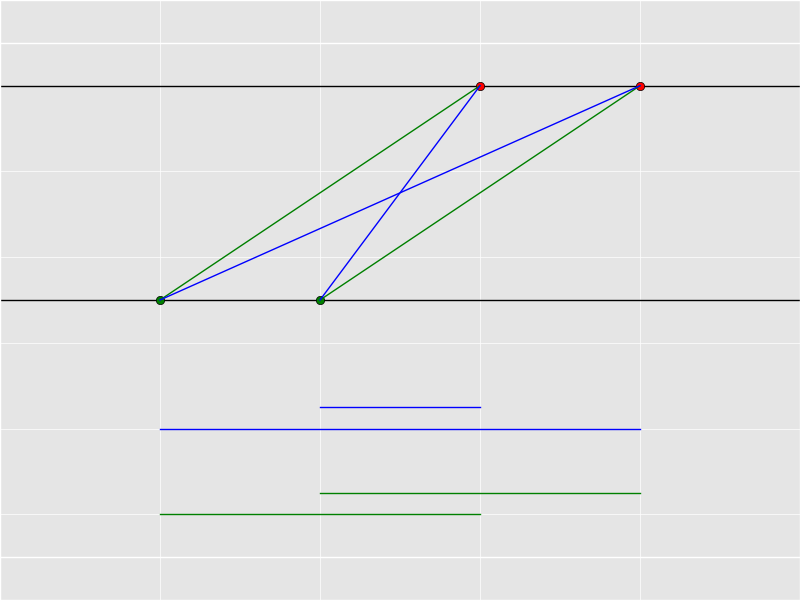
\includegraphics[width=0.5\textwidth]{demo_sort1.png}
    \caption{Graphic representation of case 1 : \emph{The upper black line represents \textbf{v} and the lower one \textbf{u}. The red points are from left to right $v_r$ and $v_q$ and The green points are from left to right $u_p$ and $u_q$. The blue lines represent what the cost when using $\sigma$ and the green lines  the cost when using $\tilde{\sigma}$. } }
\end{figure}

\begin{itemize}
	\item Case 2 : $u_p\leq v_r \leq u_q \leq v_q$
	\end{itemize}
	
	\begin{multline*}
	\begin{split}
	|u_p-v_q| + |u_q-v_r|	&\leq  |u_p-v_q|\\
		&=  v_q-u_p \\
	 	&= v_q-u_q+u_q-u_p\\
	 	&\leq v_q-u_q+v_r-u_p\\
	 	&= |u_q-v_q|+|u_p-v_r|
	\end{split}
	\end{multline*}

\begin{figure}
  \centering
    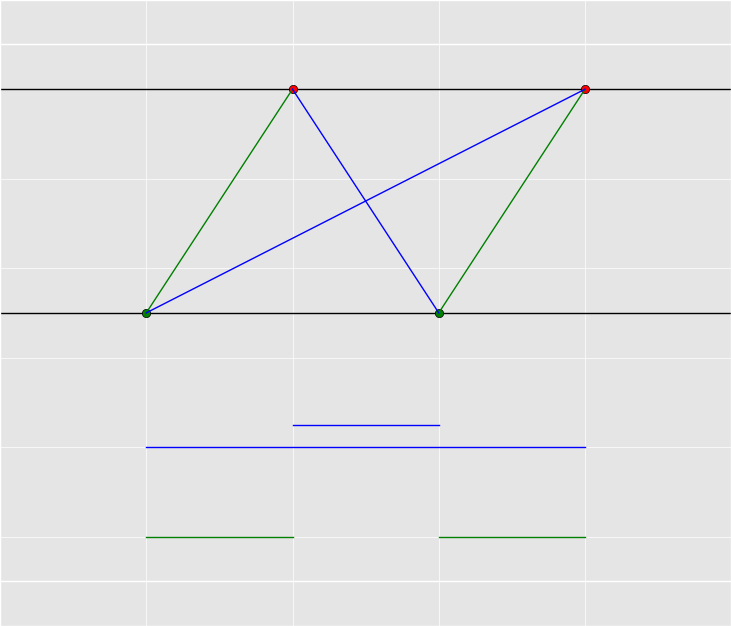
\includegraphics[width=0.5\textwidth]{demo_sort2.png}
     \caption{Graphic representation of case 2 : \emph{The upper black line represents \textbf{v} and the lower one \textbf{u}. The red points are from left to right $v_r$ and $v_q$ and The green points are from left to right $u_p$ and $u_q$. The blue lines represent what the cost when using $\sigma$ and the green lines  the cost when using $\tilde{\sigma}$. } }
\end{figure}

\begin{itemize}
	\item Case 3 : $u_p\leq v_r \leq v_q \leq u_q$
	\end{itemize}
	
\begin{figure}
  \centering
    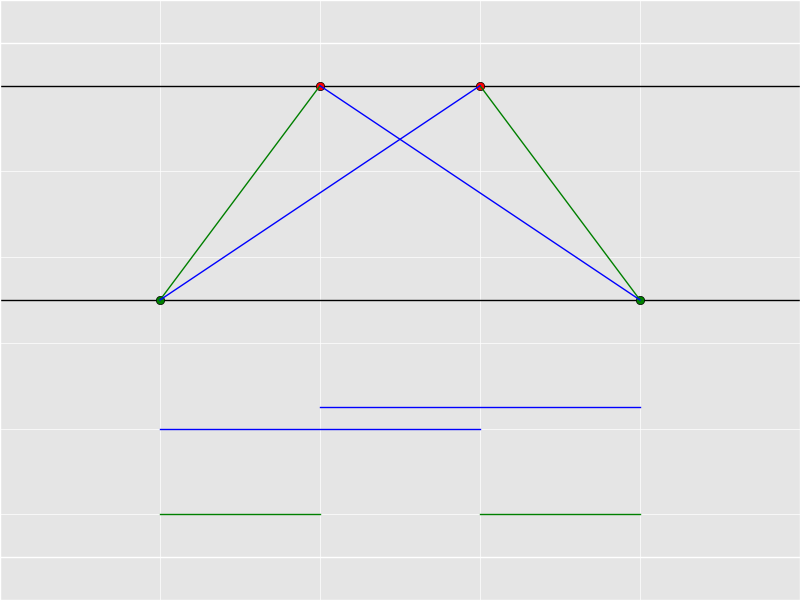
\includegraphics[width=0.5\textwidth]{demo_sort3.png}
     \caption{Graphic representation of case 3 : \emph{The upper black line represents \textbf{v} and the lower one \textbf{u}. The red points are from left to right $v_r$ and $v_q$ and The green points are from left to right $u_p$ and $u_q$. The blue lines represent what the cost when using $\sigma$ and the green lines  the cost when using $\tilde{\sigma}$. } }
\end{figure}	
	
	\begin{multline*}
	\begin{split}
	|u_p-v_q| + |u_q-v_r|	&=  v_q-u_p+u_q-v_r\\
		&=  u_q-u_p+v_q-v_r \\
	 	&\leq u_q-u_p\\
	 	&= u_q-v_q+v_q-u_p\\
	 	&\leq u_q-v_q+v_r-u_p\\
	 	&= |u_q-v_q|+|u_p-v_r|
	\end{split}
	\end{multline*}
	
	
	\begin{itemize}
	\item Case 4 : $v_r\leq v_q \leq u_p \leq u_q$\newline
	Same as case 1 by inversing the symetric roles of \textbf{u} and \textbf{v}.
	
	\item Case 5 : $v_r\leq u_p \leq v_q \leq u_q$\newline
	Same as case 2 by inversing the symetric roles of \textbf{u} and \textbf{v}.
	
	\item Case 6 : $v_r\leq u_p \leq u_q \leq v_q$\newline
	Same as case 3 by inversing the symetric roles of \textbf{u} and \textbf{v}.
	\end{itemize}

In all this cases, we have :
\begin{equation*}
	|u_p-v_q| + |u_q-v_r| \leq |u_q-v_q|+|u_p-v_r|
\end{equation*}
Let us define $\tilde{\sigma} = \sigma \circ (p q)$ :\newline
\begin{equation*}
 	\forall i \notin \{p,q\}, \tilde{\sigma} (i)=\sigma (i)
\end{equation*}
\begin{equation*}
 	\tilde{\sigma} (p)=r
\end{equation*}
\begin{equation*}
 	\tilde{\sigma} (q)=q
\end{equation*}

Then  we have

\begin{multline*}
	\begin{split}
	\sum_{i=1}^n |u_i-v_{\sigma (i)}|	&= \sum_{i\notin \{p,q\}} |u_i-v_{\sigma (i)}|+|u_p-v_q|+|u_q-v_r|\\
	 	&\leq \sum_{i\notin \{p,q\}} |u_i-v_{\sigma (i)}|+|u_q-v_q|+|u_p-v_r|\\
	 	&=\sum_{i=1}^n |u_i-v_{\tilde{\sigma} (i)}|
	\end{split}
	\end{multline*}

So, $\tilde{\sigma}$ reaches the minimum too and $supp(\tilde{\sigma}) = supp(\sigma) \setminus \{\max supp(\sigma) \}$. By doing this operation many times, we can remove all the elements of $supp(\sigma)$. So Id reaches the minimum. $\Box$
	
	
\end{document}